%!TEX program = xelatex
%!TEX TS-program = xelatex
%!TEX encoding = UTF-8 Unicode

\documentclass{article} % For LaTeX2e
\usepackage{iclr2017_conference,times}
%\usepackage{hyperref}
\usepackage{url}
\renewcommand\refname{参考文献}
\renewcommand\bibname{参考文献}

\usepackage[UTF8, heading = false, scheme = plain]{ctex}

\usepackage[english]{babel}
\usepackage[utf8]{inputenc}
\usepackage{fancyhdr,graphicx,amsmath,amssymb,subcaption}
\usepackage[ruled,vlined]{algorithm2e}
\usepackage{multirow}
\usepackage{wrapfig}

\newcommand*{\eg}{e.g.\@\xspace}
\newcommand*{\ie}{i.e.\@\xspace}
\newcommand*{\wrt}{w.r.t.\@\xspace}
\newcommand*{\st}{s.t.\@\xspace}
\newcommand*{\eq}{Eq.\@\xspace}
\newcommand*{\vs}{vs.\@\xspace}
\newcommand*{\incl}{incl.\@\xspace}
\newcommand*{\apprx}{approx.\@\xspace}
\newcommand*{\registered}{{\ooalign{\hfil\raise .00ex\hbox{\scriptsize R}\hfil\crcr\mathhexbox20D}}\@\xspace}

\hyphenation{hyper-para-meters}

\title{使用图卷积网络进行半监督分类}

\author{Thomas N. Kipf\\
阿姆斯特丹大学 \\
\texttt{T.N.Kipf@uva.nl} \\
\And
Max Welling\\
阿姆斯特丹大学 \\
加拿大高等研究院 (CIFAR)\\
\texttt{M.Welling@uva.nl} \\
}

\newcommand{\fix}{\marginpar{FIX}}
\newcommand{\new}{\marginpar{NEW}}

\iclrfinalcopy

\begin{document}

\maketitle

\vskip.075in\centerline{\large 摘要}\vspace{0.5ex}\begin{quote}
我们展现了一种可扩展的用于图上数据的半监督学习方法,这一方法是基于卷积网络的一种可直接在图上使用的高效变体。我们从谱图卷积的局部一阶近似推导出我们的卷积结构。我们的模型随着图上边的个数以及隐藏层线性增大。这种隐藏层编码了图的局部信息以及节点的特征。通过一些引用网络的和知识图谱的实验,我们证明了我们的方法显著好于其他方法。
\par\end{quote}\vskip 1ex

\section{引言}
我们来考虑图(比如引用网络)上节点(比如文章)的分类问题,并且假定只有相当少的节点已知类别(标签)。这个问题可以被归结为图上的半监督学习。类别信息可以通过显式的基于图结构的正则化来进行平滑 \citep{zhu2003semi, zhou2004learning, belkin2006manifold, weston2012deep},比如使用在损失函数中使用图拉普拉斯正则项:
\begin{equation}
  \mathcal{L} = \mathcal{L}_0 + \lambda \mathcal{L}_{\text{reg}}\, , \quad \text{其中} \quad \mathcal{L}_{\text{reg}}= \sum_{i,j}A_{ij}\Vert f(X_i)-f(X_j) \Vert ^2 = f(X)^\top \Delta f(X) \, .
\label{eq:graph-reg}
\end{equation}
这里, $\mathcal{L}_0$ 代表有监督的损失,对应着已知类别的节点, $f(\cdot)$ 可以是类似神经网络的可微函数, $\lambda$ 是一个权重因子,$X$ 是由节点特征向量 $X_i$ 组成的矩阵。 无向图$\mathcal{G}=(\mathcal{V}, \mathcal{E})$,具有 $N$ 个节点 $v_i \in \mathcal{V}$, 边 $(v_i, v_j)\in\mathcal{E}$, 以及邻接矩阵 $A\in\mathbb{R}^{N\times N}$(二值或者有权)以及度矩阵 $D_{ii} = \sum_j A_{ij}$。 公式中的$\Delta = D - A$ 表示未经标准化的图拉普拉斯矩阵。公式\eqref{eq:graph-reg}依赖于“图上邻接的节点更有可能属于同一类”的假设。然而,这一假设会限制模型的能力,因为图上的边不一定编码节点的相似性,有可能代表其他信息。

在这个工作证,我们直接使用神经网络 $f(X, A)$ 来编码图结构,然后直接用所有有标签的节点来训练有监督的目标函数 $\mathcal{L}_0$,因此避免了损失函数中显式的基于图的正则项。把邻接矩阵作为$f(\cdot)$的一个变量,使得模型可以把梯度信息从有监督的损失 $\mathcal{L}_0$ 分散开来,以至于无论有无标签,都能够学习出一个节点的表示向量。

我们的贡献分为两个部分。首先,我们为神经网络引入了一个简单但是有效的分层传播规则,使得它可以直接作用于图上。我们展示了这个规则是如何从一个特殊的谱图卷积\citep{hammond2011wavelets}的一阶近似导出。其次,我们展示了这种基于图的神经网络模型是如何被用于快速的可扩展的图上节点半监督分类问题。在数个数据集上的实验都说明了我们的模型在分类精度和效率上能够比肩最顶尖的无监督算法。

\section{图上快速近似卷积}
\label{sec:fast-convs}

这一节,我们提供本文即将用的基于图的神经网络模型 $f(X, A)$ 的理论来源。我们考虑一个有着如下传播规则的多层图卷积网络 (Graph Convolutional Network,GCN)。
\begin{equation}
  \textstyle
  H^{(l+1)}= \sigma\!\left(\tilde{D}^{-\frac{1}{2}} \tilde{A}\tilde{D}^{-\frac{1}{2}}H^{(l)} W^{(l)} \right) \, .
\label{eq:gcn-layer}
\end{equation}
这里,$\tilde{A} = A + I_N$ 代表着手动增加自环的无向图 $\mathcal{G}$ 的邻接矩阵,$I_N$ 是单位矩阵,$\tilde{D}_{ii} = \sum_j \tilde{A}_{ij}$, $W^{(l)}$ 是本层可训练的权值矩阵, $\sigma(\cdot)$ 是激励函数,比如$\mathrm{ReLU}(\cdot) = \max(0,\cdot)$。 $H^{(l)}\in \mathbb{R}^{N\times D}$ 是神经网络第$l$层节点的激励值,且 $H^{(0)}=X$ 。接下来,我们会说明这种形式的传播规则可以通过图上的局部谱滤波\citep{hammond2011wavelets, defferrard2016convolutional}的一阶近似导出。

\subsection{谱图卷积}
图上的谱卷积被定义为一个图信号 $x\in \mathbb{R}^N$ (每个节点对应一个标量)和一个在傅里叶空间里具有参数 $\theta\in \mathbb{R}^N$ 的滤波模板 $g_{\theta}=\text{diag}(\theta)$ 的乘积:
\begin{equation}
  g_{\theta} \star x =  Ug_{\theta}U^\top x \, ,
\label{eq:fourier-conv}
\end{equation}
其中 $U$ 是标准化的图拉普拉斯矩 $L = I_N - D^{-\frac{1}{2}}AD^{-\frac{1}{2}} = U\Lambda U^\top$ 的阵特征向量, $\Lambda$ 是其特征值组成的对角阵, $U^\top x$ 代表图信号$x$的傅立叶变换结果。我们可以把 $g_{\theta}$ 理解为一个关于 $L$ 特征值的函数,比如 $g_{\theta}(\Lambda)$。 公式\ref{eq:fourier-conv}的计算复杂度很高,因为与特征向量 $U$ 的乘法是 $\mathcal{O}(N^2)$ 的。除此之外,计算 $L$ 的特征值分解对于大型的图也是无法接受的。为了解决这些问题, \cite{hammond2011wavelets}中提到 $g_{\theta}(\Lambda)$可以被产开成 $K$ 阶契比雪夫多项式的和:
\begin{equation}
  g_{\theta'}(\Lambda) \approx \sum_{k=0}^{K} \theta_k ' T_k(\tilde{\Lambda}) \, ,
\label{eq:tchebyshew}
\end{equation}
其中 $\tilde{\Lambda}=\frac{2}{\lambda_{\text{max}}}\Lambda-I_N$,是缩放过的特征值矩阵。 $\lambda_{\text{max}}$ 代表 $L$ 最大的特征值. $\theta'\in \mathbb{R}^K$ 是系数 $\theta'_k$ 组成的向量。 切比雪夫多项式被递归的定义为 $T_k(x) = 2xT_{k-1}(x) - T_{k-2}(x)$, 特殊的 $T_0(x)=1$ 且 $T_1(x)=x$. 读者可以参考 \cite{hammond2011wavelets} 详细了解这个近似.

回到我们对在 $x$ 上作用卷积核 $g_{\theta'}$ 的定义, 我们现在有:
\begin{equation}
  g_{\theta'} \star x \approx  \sum_{k=0}^{K} \theta_k' T_k(\tilde{L}) x \, ,
\label{eq:fourier-conv-approx}
\end{equation}
其中 $\tilde{L} = \frac{2}{\lambda_{\text{max}}}L-I_N$;观察到$(U\Lambda U^\top)^k = U \Lambda^k U^\top$,这个可以很容易验证。 注意到这个公式目前是 $K$ 局部化的。 因为它是拉普拉斯矩阵的 $K$ 阶多项式,也就是说它只依赖于距离中心节点 $K$ 步以内的节点 ($K$阶邻居). 计算公式 \ref{eq:fourier-conv-approx} 的复杂度为 $\mathcal{O}(|\mathcal{E}|)$,即随边数线性增长。 \cite{defferrard2016convolutional} 就使用这种 $K$局部化的卷积定义了一个图上的卷积神经网络。

\subsection{分层线性模型}
\label{sec:linear-model}
之后通过不断的堆叠形如公式\ref{eq:fourier-conv-approx}的卷积层且每层最后进行激活,就可以构建出一个神经网络。现在,想象我们限制每层的卷积操作的阶数 $K=1$ (见公式 \ref{eq:fourier-conv-approx}),即一个 $L$ 的线性函数,也是一个关于图拉普拉斯矩阵的特征值的线性函数。

通过这种方法,我们仍然可以通过堆叠卷积层获得丰富的卷积函数,但是我们没有被要求只能使用显式的正则项,如切比雪夫多项式。我们直觉上期望这个模型可以缓解在节点度变化很大的图上,如社交网络,引用网络,知识图谱以及许多其他真是世界的网络,对局部邻居结构的过拟合问题。除此之外,在计算能力有限的情况下,这种分层的公式允许我们构建更深的模型,这是一个常用的提升模型能力的做法\citep{he2015deep}。

在这个图卷积网络的线性公式中,我们更近一步令 $\lambda_{\text{max}}\approx 2$ ,因为我们知道神经网络在训练中会自动适应这个缩放上的变化。 在这些近似下公式\ref{eq:fourier-conv-approx}简化为:
\begin{equation}
  g_{\theta'} \star x \approx  \theta_0' x
  + \theta_1' \left(L-I_N\right)x = \theta_0' x - \theta_1' D^{-\frac{1}{2}}AD^{-\frac{1}{2}} x \, ,
\label{eq:fourier-conv-approx2}
\end{equation}

带有两个自由变量 $\theta_0'$ 与 $\theta_1'$。 这两个卷积参数可以在整张图上共享。 连续使用这种形式的滤波器可以高效的对一个节点的 $k$ 阶邻居进行卷积, $k$ 是连续卷积操作的数量,或者是神经网络中卷积层的个数。

实践中,限制参数个数可以有效的解决过拟合问题,并且减小每一层的计算量。所以我们提出如下公式:
\begin{equation}
  g_{\theta} \star x \approx  \theta \left(I_N + D^{-\frac{1}{2}}AD^{-\frac{1}{2}}\right) x \, ,
\label{eq:fourier-conv-approx3}
\end{equation}
只带有个一参数 $\theta = \theta_0'=-\theta_1'$。注意到现在 $I_N + D^{-\frac{1}{2}}AD^{-\frac{1}{2}}$ 的特征值都在区间 $[0, 2]$ 内。在深层网络中不停的重复这一操作,会导致数值上的不稳定以及梯度爆炸或者梯度消失问题。为了缓解这一问题,我们引入 \textit{再标准化技巧}:
$I_N + D^{-\frac{1}{2}}AD^{-\frac{1}{2}}\rightarrow \tilde{D}^{-\frac{1}{2}}\tilde{A}\tilde{D}^{-\frac{1}{2}}$, 其中 $\tilde{A} = A + I_N$ 且 $\tilde{D}_{ii} = \sum_j \tilde{A}_{ij}$.

我们可以把这个定义推广到一个有着 $C$ 个通道的信号  $X\in\mathbb{R}^{N\times C}$(即每个节点都有一个 $C$ 维的特征向量)和 $F$ 个卷积核做卷积:
\begin{equation}
  Z = \tilde{D}^{-\frac{1}{2}}\tilde{A}\tilde{D}^{-\frac{1}{2}}X\Theta \, ,
\label{eq:fourier-conv-approx4}
\end{equation}
其中 $\Theta\in\mathbb{R}^{C\times F}$ 现在是由卷积参数组成的一个矩阵,并且 $Z\in\mathbb{R}^{N\times F}$ 卷积结果。 这个卷积操作的复杂度为 $\mathcal{O}(|\mathcal{E}|FC)$,因为 $\tilde{A}X$ 是稀疏矩阵和稠密矩阵的乘积。

\section{半监督节点分类}
在介绍完了能够在图上进行高效信息传播的简单但是灵活的模型 $f(X,A)$ 之后,我们可以回到半监督节点分类问题上来。就像引言中概述的那样,通过把数据 $X$ 和代表图结构的邻接矩阵 $A$ 都作为 $f(X,A)$ 的输入,我们可以放宽图上半监督学习常做的一些假设。 我们期待这种放宽可以在邻接矩阵包含 $X$ 所不具备的信息时,有着特别的效果。图\ref{fig:model}刻画了一个用于半监督学习的多层图卷积网络的大致结构。

\begin{figure}[htp]
    \centering
    \begin{subfigure}[b]{0.67\textwidth}
        \centering
    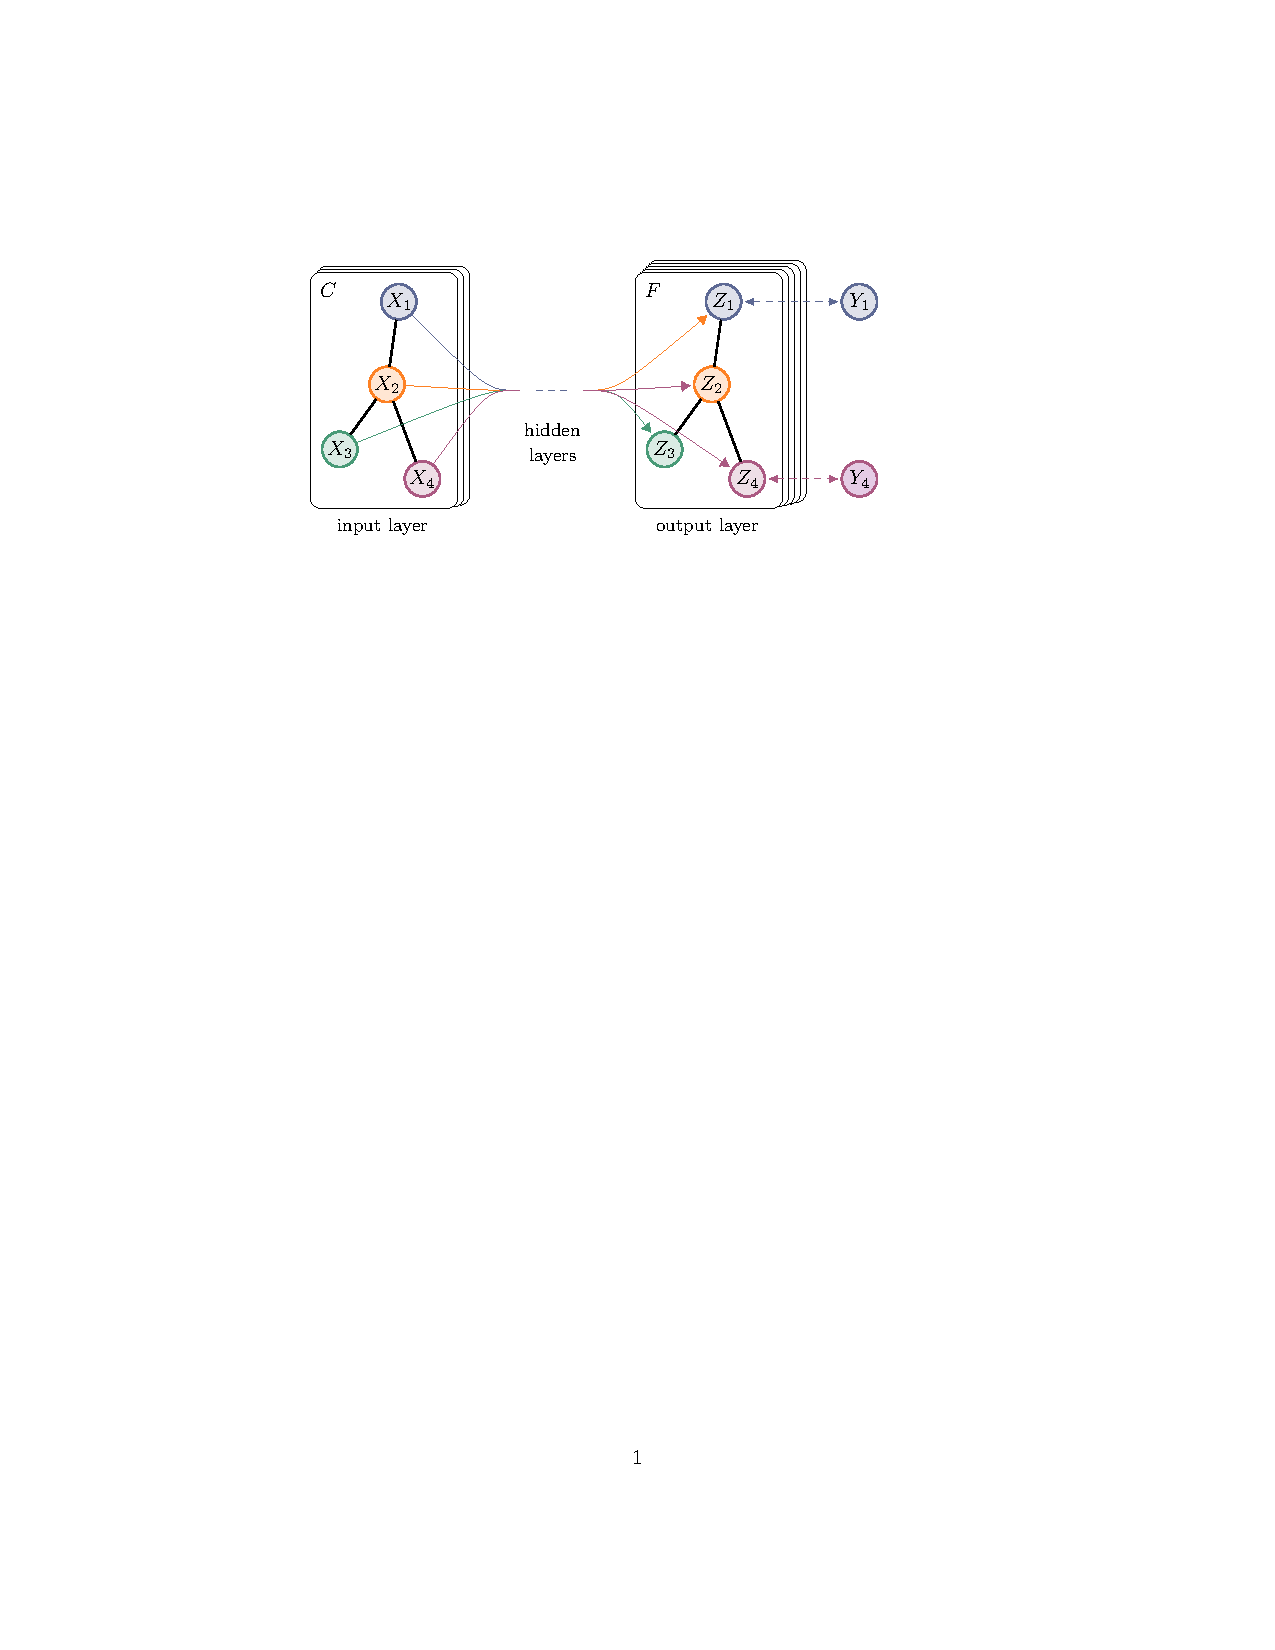
\includegraphics[clip, trim=5cm 18.8cm 6.4cm 4.4cm, width=\textwidth]{graph_simple.pdf}
        \caption{图卷积网络}
        \label{fig:model-a}
    \end{subfigure}%
    ~
    \begin{subfigure}[b]{0.33\textwidth}
        \centering
        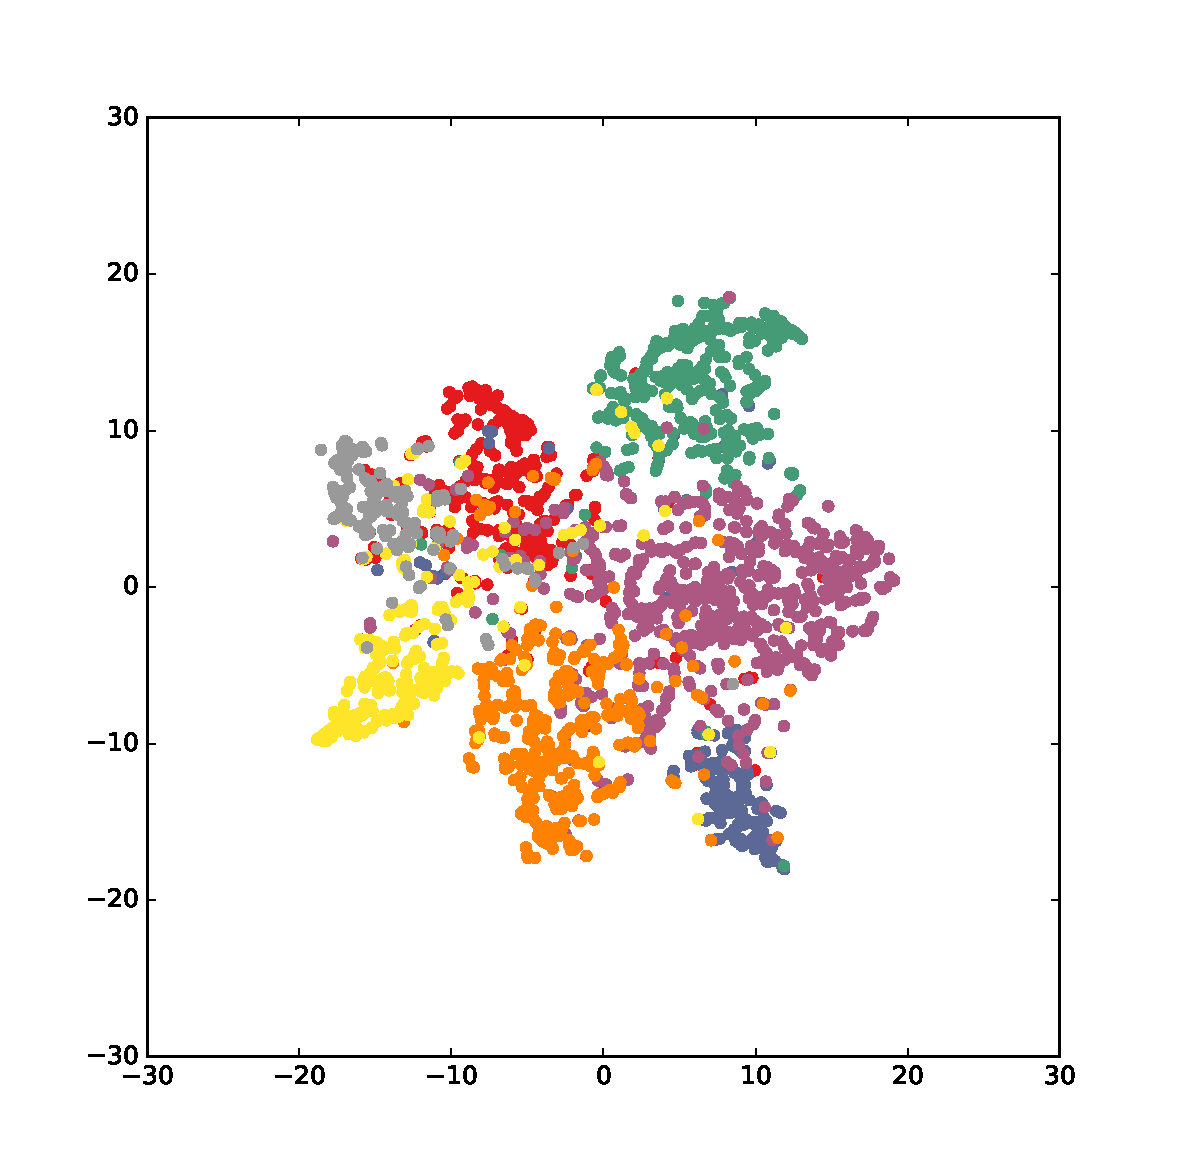
\includegraphics[width=\textwidth, trim={4cm 4cm 4cm 4cm}, clip]{tsne_cora_6.pdf}
        \caption{隐藏层的值}
        \label{fig:model-b}
    \end{subfigure}

    \caption{\emph{左图}:用于半监督学习,输入特征具有 $C$ 个通道,输出具有 $F$ 类的多层图卷积网络的结构。图结构 (黑线代表边) 在每一层都是共享的, $Y_i$ 代表标签。\emph{右图}:两层图卷积网络的隐藏层的t-SNE \citep{maaten2008visualizing} 可视化结果。训练集为 Cora 数据集 \citep{sen2008collective},仅用了 $5\%$ 的标签。颜色表示类别。}
    \label{fig:model}
\end{figure}

\subsection{实例} \label{sec:model-example} 接下来,我们考虑一个两层的图卷积网络,应用于半监督图上节点分类问题,图有对称的邻接矩阵 $A$ (二值或者有权)。我们首先在预处理中计算 $\hat{A} = \tilde{D}^{-\frac{1}{2}}\tilde{A}\tilde{D}^{-\frac{1}{2}}$。我们的模型有着如下的简单形式:
\begin{equation}
Z= f(X,A) =  \mathrm{softmax}\!\left(\hat{A} \,\, \mathrm{ReLU}\!\left(\hat{A} X W^{(0)} \right) W^{(1)} \right) \, .
\label{eq:two-layer-gcn}
\end{equation}
这里, $W^{(0)}\in \mathbb{R}^{C\times H}$ 输入层到有 $H$ 维的隐藏层的权值矩阵。$W^{(1)}\in \mathbb{R}^{H\times F}$ 是隐藏层到输出层的权值矩阵。softmax激励函数, 定义为 $\mathrm{softmax}(x_i)=\frac{1}{\mathcal{Z}}\exp(x_i)$ 其中 $\mathcal{Z}=\sum_i \exp(x_i)$,将会作用于每一行。 对于半监督多分类问题, 我们将计算在所有有标签数据上的交叉熵误差:
\begin{equation}
\mathcal{L}= -\sum_{l\in\mathcal{Y}_L}\sum_{f=1}^F Y_{lf} \ln Z_{lf}  \, ,
\label{eq:}
\end{equation}
这里 $\mathcal{Y}_L$ 是所有有标签节点的下标。

神经网络权重 $W^{(0)}$ 和 $W^{(1)}$ 使用梯度下降来进行训练。 在本文中,我们的每次迭代都会使用整个数据集, 在整个数据集可以放入内存时,这确实是一个可行的选项。 如果使用 $A$ 稀疏表示, 内存要求为 $\mathcal{O}(|\mathcal{E}|)$, 是边个数的线性函数。 训练过程中使用 dropout \citep{srivastava2014dropout}。 更加节省内存的随机梯度下降将会在未来的工作中实现。

\subsection{实现} 实践中,我们使用 tensorflow  \citep{tensorflow2015-whitepaper} 中的稀疏矩阵乘法来高效的实现公式 \ref{eq:two-layer-gcn} 的 GPU 版本 \footnote{重复我们结果的代码可以在 \url{https://github.com/tkipf/gcn} 中找到。}。 那么公式 \ref{eq:two-layer-gcn} 的计算复杂度为 $\mathcal{O}(|\mathcal{E}|CHF)$,即随边个数线性增长。


\section{相关工作}
我们的模型主要是受到了图上半监督学习和图上神经网络中受到了启发。接下来,我们将会简短回顾一下这两个领域的相关工作。

\subsection{图上半监督学习}
最近几年提出了大量的基于图的半监督学习方法,它们大致可以分为两类:显式使用图拉普拉斯正则化的方法和基于embedding的方法。重要的使用图拉普拉斯正则化的例子包括标签传播 \citep{zhu2003semi},流形正则化 \citep{belkin2006manifold},以及深度半监督embedding \citep{weston2012deep}。%These approaches have been extended with ideas from spectral graph theory \citep{shuman2011semi, ekambaram2013wavelet}.

最近,焦点已经转移到了用类似skip-gram模型 \citep{mikolov2013distributed} 的方法学习图的embedding。DeepWalk \citep{perozzi2014deepwalk} learns embeddings 通过预测节点的局部邻居来学习embedding,这些邻居通过图上随机游走来采样。LINE \citep{tang2015line} 和 node2vec \citep{grovernode2vec} 用更复杂的随机游走或者宽度优先搜索扩展了 DeepWalk。然而所有的这些方法分为多个步骤,包括随机游走生成和半监督训练,每一步都要单独优化。Planetoid \citep{yang2016revisiting} 通过在训练步骤中注入标签信息缓解了这个问题.


\subsection{图上神经网络} \cite{gori2005new, scarselli2009graph} 之前曾以一种循环神经网络的形式引入了图上的神经网络。他们的框架要求重复作用压缩映射作为传播函数,直到节点的表示向量达到稳定。这个限制之后在 \cite{li2015gated} 中放宽了,把了现代循环神经网络中常用的技巧引入了之前的图神经网络框架。 \cite{duvenaud2015convolutional} 介绍了一种类似卷积的规则来进行整个图的分类。他们的方法需要针对不同的度学习不同的权值矩阵,并不能很好的应用于度变化很大的大型图。相比之下,我们的模型每一层使用一个相同的权值矩阵,通过适当标准化邻接矩阵来解决度的变化问题。(见本文\ref{sec:model-example}).

最近\cite{atwood2016diffusion}介绍了一个使用图上神经网络进行节点分类的方法。他们的方法具有 $\mathcal{O}(N^2)$ 的复杂度,限制了可能的应用范围。在另一个不同的模型中, \cite{niepert2016learning} 把图的局部转换成了序列然后送入了使用一维离散卷积的神经网络中, 这需要在预处理中定义节点顺序.

我们的方法基于谱图卷积神经网络,由 \cite{bruna2014spectral} 引进并由\cite{defferrard2016convolutional}通过快速局部卷积扩展。与这些工作不同的是,我们这里考虑了大规模网络的转导式的节点分类任务。我们展示了在这种情况下,一定数量的简化(见本文\ref{sec:linear-model})可以被引入到\cite{bruna2014spectral} 和 \cite{defferrard2016convolutional} 原本的框架中,以提高可扩展性以及在大规模网络上的效果。

\section{实验}
我们针对我们的模型进行了许多实验:引用网络上的半监督文本分类,从知识图谱上抽取的二分图的实体分类,各种图传播模型的比较,随机图上的运行时间分析。


\subsection{数据集}
\label{sec:datasets}
我们紧随 \cite{yang2016revisiting} 中设计的实验。 数据集的统计信息总结在表\ref{tab:datasets}. 在引用网络数据集中---Citeseer,Cora 和 Pubmed \citep{sen2008collective}---节点代表文献,边代表引用。 标签比例代表带有标签的节点比例。 NELL \citep{carlson2010toward, yang2016revisiting} 是一个二分图,从一个有55,864种关系,9,891个实体的知识图谱中抽取出来。

\begin{table}[htp]
\centering
\caption{\label{tab:datasets}数据集统计信息,由 \cite{yang2016revisiting}提供}
\begin{tabular}{l c r r r r r}
\textbf{数据集} & \textbf{类型} & \textbf{节点} & \textbf{边} & \textbf{类别} & \textbf{特征} & \textbf{标签比例}  \\[0.05em]\hline \\[-0.8em]
Citeseer & 引用网络 & 3,327 & 4,732 & $6$ & 3,703 & $0.036$ \\
Cora & 引用网络 & 2,708 & 5,429 & $7$ & 1,433 & $0.052$ \\
Pubmed & 引用网络& 19,717 & 44,338 & $3$ & 500 & $0.003$ \\
NELL & 知识图谱 & 65,755 & 266,144 & $210$ & 5,414 & $0.001$ \\
\end{tabular}
\end{table}

\paragraph{引用网络} 我们考虑三个引用网络数据集:Citeseer,Cora 和 Pubmed \citep{sen2008collective}。数据集包含了每篇文献的词袋(bag of word)特征以及文献之间的引用关系。我们把引用关系当做图上的无向边,构造了一个二值且对称的邻接矩阵 $A$。每个文献有一个类型标签。训练时,我们每类只用了20个有标签的数据,但是所有节点的特征向量我们都会使用。

\paragraph{NELL} NELL 是从 \citep{carlson2010toward} 所介绍的知识图谱中抽取出来的一个数据集。知识图谱是一个有向图,但是每个边具有标签,代表不同的关系。 追随 \cite{yang2016revisiting} 中介绍的预处理技术,我们为每一个实体关系三元组 $(e_1, r, e_2)$ 在图上增加节点 $r_1$ 和 $r_2$,和边$(e_1, r_1)$ 及 $(e_2, r_2)$。实体节点具有稀疏的特征向量。我们给每个关系节点赋上一个唯一的 one-hot 向量,因此把特征的维度扩展到了61,278(关系种类+原有的特征维度)。这里的半监督任务考虑最极端的情况,每一类只有一个有标记的数据。如果两个节点$i$ 和 $j$ 之间有边,就设置$A_{ij}=1$。
这样我们就构造了一个二值,对称的邻接矩阵。

\paragraph{随机图} 为了进行运行速度的比较,我们构造了许多随机图。对于一个有 $N$ 个节点的图,我们均匀随机添加 $2N$ 个边。我们把单位矩阵 $I_N$ 作为输入的特征矩阵 $X$,因此隐式的使用了一种无特征的方法,算法仅仅知道由独一无二的one-hot向量提供的每个节点的id。对每个节点,我们都给相同的标签 $Y_i = 1$。

\subsection{实验设计}
除非另有说明,我们训练的都是\ref{sec:model-example}中描述的双层的图卷积网络,然后在1000个数据点的训练集上进行测试。附录\ref{sec:depth}我们提供额外的使用深达10层的网络的实验。我们与 \cite{yang2016revisiting} 选择相同的数据集分割,但是有额外的500个数据点构成验证集用于超参数的优化(dropout概率,L2正则化系数,隐藏层个数)。训练时并不会用到验证集的标签。

对于引用网络,我们会在仅在Cora上调整超参数,然后直接用于Citeseer和Pubmed数据集。模型最多训练200个轮(epoch),使用Adam优化器 \citep{kingma2014adam},学习速率为 $0.01$,使用窗口大小为 $10$ 的提前停止机制。权制根据 \cite{glorot2010understanding} 中描述当方法进行初始化,并且对特征对每一行进行标准化。对于随机图数据集,我们使用32个节点的隐藏层,而且省略了正则化(比如dropout或L2正则化)。

\subsection{实验基准}
我们与\cite{yang2016revisiting}使用相同的算法作为基准,来比较我们的算法。这些作为基准的算法有:标签传播(label propagation,LP)\citep{zhu2003semi}, 半监督嵌入(SemiEmb)\citep{weston2012deep},流形正则(ManiReg)\citep{belkin2006manifold} 和基于 skip-gram 的图嵌入\citep{perozzi2014deepwalk}。
我们省略了TSVM \citep{joachims1999transductive},因为它并不适用于节点类型很多的数据集(NELL)。

我们更进一步的和\cite{lu2003link}提出的迭代分类算法(ICA)与两个逻辑回归分类器的结合做了比较,一个只用节点特征,另一个使用图的局部特征和\cite{sen2008collective}中提出的增强算子。

最后,我们和 Planetoid \citep{yang2016revisiting}做了比较,我们总是把他们效果最好的模型变体(转导或者直推)用作比较的基准。

\section{结果}
\label{sec:results}

\subsection{半监督节点分类}
表 \ref{tab:results_node} 总结了所有的结果。数字代表分类正确率。对于ICA,我们报告了他们100次运行的平均准确率,每次运行都对节点顺序进行随机。其他算法的结果都出自 Planetoid 的论文 \citep{yang2016revisiting}. Planetoid* 代表对应数据集上该模型效果最好的变体。

\begin{table}[htp]
\centering
\caption{\label{tab:results_node}分类准确率 (百分比)}
\begin{tabular}{l l l l l}
\textbf{方法} & \textbf{Citeseer} & \textbf{Cora} & \textbf{Pubmed} & \textbf{NELL} \\[0.05em]\hline \\[-0.8em]
ManiReg [\citenum{belkin2006manifold}] & $60.1$ & $59.5$ & $70.7$ & $21.8$ \\
SemiEmb [\citenum{weston2012deep}] & $59.6$ & $59.0$ & $71.1$ & $26.7$ \\
LP [\citenum{zhu2003semi}] & $45.3$ & $68.0$ & $63.0$ & $26.5$ \\
DeepWalk [\citenum{perozzi2014deepwalk}] & $43.2$ & $67.2$ & $65.3$ & $58.1$ \\
ICA [\citenum{lu2003link}] & $69.1$ & $75.1$ & $73.9$ & $23.1$ \\
Planetoid* [\citenum{yang2016revisiting}] & $64.7$ (26s) & $75.7$ (13s) & $77.2$ (25s) & $61.9$ (185s) \\
\textbf{GCN} (this paper) & $\mathbf{70.3}$ (7s) & $\mathbf{81.5}$ (4s) & $\mathbf{79.0}$ (38s) & $\mathbf{66.0}$ (48s) \\[0.05em]\hline \\[-0.8em]
GCN (rand.\@\xspace splits) & $67.9 \pm 0.5$ & $80.1 \pm 0.5$ & $78.9 \pm 0.7$ & $58.4 \pm 1.7$ \\
\end{tabular}
\end{table}

我们进一步统计了我们这个模型和Planetoid模型从开始到收敛的训练时间(写在括号内的)。对于后者,我们使用原作者的代码\footnote{\url{https://github.com/kimiyoung/planetoid}}, 并与我们的GCN模型使用相同的机器配置。 我们使用与\cite{yang2016revisiting}相同的书数据集划分来训练我们的模型,并且报告100次运行的平均准确度,每次运行都随机初始化权值。我们在 Citeseer, Cora and Pubmed 上使用相同的超参数:0.5(dropout 概率),$5\cdot 10^{-4}$(L2 正则系数)和 $16$(隐藏层节点个数); 对于 NELL: 0.1(dropout 概率),$1\cdot 10^{-5}$(L2 正则系数)和 $64$ (隐藏层节点个数)。

除此之外,我们像\cite{yang2016revisiting}一样报告了我们模型在数据集的10个随机划分上的的效果,记为GCN (rand.\@\xspace splits)。这里,我们报告预测准确率的均值和标准差。

\subsection{传播模型的评估}
我们比较了我们提出的分层传播模型在引用网络上的各种变体。我们追随前一章节的实验设计。结果写在表 \ref{tab:results_model_eval}。我们原版GCN模型的传播方式被记为\textit{再标准化技术}(粗体)。其他模型中,神经网络的传播方式都列在\textit{传播方式}一栏。右边的数字代表100次随机初始化重复运行的平均分类正确率。在每层有多个参数 $\Theta_i$ 的时候,我们给第一层的权值矩阵加入 L2 正则化。

\begin{table}[htp]
\centering
\caption{\label{tab:results_model_eval}传播方式比较}
\begin{tabular}{l c c r r r}
\textbf{名字} & & \textbf{传播方式} & \textbf{Citeseer} & \textbf{Cora} & \textbf{Pubmed} \\[0.05em]\hline \\[-0.8em]

\multirow{2}{*}{切比雪夫滤波器 (公式 \ref{eq:fourier-conv-approx})} & $K=3$  & \multirow{2}{*}{$\sum_{k=0}^K  T_k(\tilde{L}) X \Theta_k$} & $69.8$& $79.5$ & $74.4$    \\
  & $K=2$ &  & $69.6$& $81.2$ & $73.8$    \\[0.05em]\hline \\[-0.9em]
\multicolumn{2}{l}{$1^{\text{st}}$阶模型 (公式 \ref{eq:fourier-conv-approx2})}  & $X\Theta_0 + D^{-\frac{1}{2}}AD^{-\frac{1}{2}}X\Theta_1$ & $68.3$& $80.0$ & $77.5$ \\
\multicolumn{2}{l}{单参数 (公式 \ref{eq:fourier-conv-approx3})} & $(I_N + D^{-\frac{1}{2}}AD^{-\frac{1}{2}})X\Theta$ & $69.3$& $79.2$ & $77.4$ \\
\multicolumn{2}{l}{\textbf{再标准化技术} (公式 \ref{eq:fourier-conv-approx4})}& $\tilde{D}^{-\frac{1}{2}}\tilde{A}\tilde{D}^{-\frac{1}{2}}X\Theta$ & $\mathbf{70.3}$ & $\mathbf{81.5}$ & $\mathbf{79.0}$   \\[0.25em]\hline \\[-0.9em]
\multicolumn{2}{l}{仅用$1^{\text{st}}$阶项}
 & $D^{-\frac{1}{2}}AD^{-\frac{1}{2}}X\Theta$ & $68.7$ & $80.5$ & $77.8$ \\
\multicolumn{2}{l}{多层感知机} & $X\Theta$ & $46.5$ & $55.1$ & $71.4$ \\
\end{tabular}
\end{table}

\newpage
\subsection{每轮训练时间}
\begin{wrapfigure}{r}{0.5\textwidth}
\vspace{-3em}
    \centering
    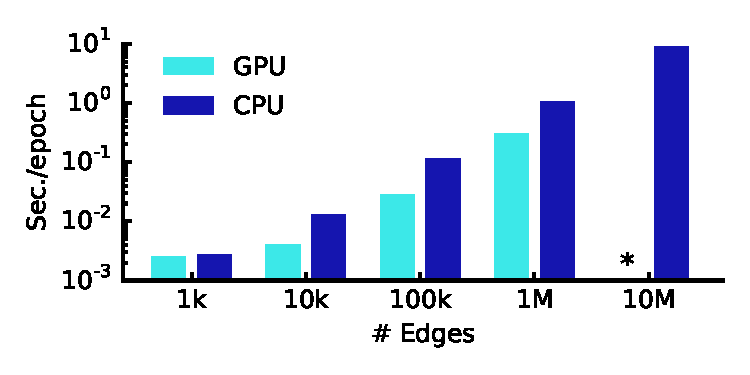
\includegraphics[scale=0.56, trim={0.45cm 0.45cm 0.45cm 0}, clip]{time_per_epoch}
    \caption{随机图上每轮训练的挂钟时间(Wall-clock time)。 (*) 代表内存溢出。}
    \label{fig:epoch_timing}
    \vspace{-1em}
\end{wrapfigure}

这里我们报告了每轮的平均训练时间(正向传播,交叉熵计算,反向传播)。每个在随机生成的图上训练100轮,用挂钟时间作为评价指标。本文 \ref{sec:datasets} 有生成随机图的详细说明。我们比价了GPU和CPU版本的运行速度\footnote{硬件: 16-core Intel\registered Xeon\registered CPU E5-2640 v3 @ 2.60GHz, GeForce\registered GTX TITAN X} in TensorFlow \citep{tensorflow2015-whitepaper}。 图 \ref{fig:epoch_timing} 给出最后结果。
%\vspace{4em}

\section{讨论}

\subsection{半监督模型}
从以上实验中可以看出,我们提出的进行半监督节点分类的方法明显好于最近的相关算法。基于图拉普拉斯正则化 \citep{zhu2003semi, belkin2006manifold, weston2012deep} 的方法受限最严重,因为它假设边仅仅表示节点相似度。另一方面,基于Skip-gram的方法则受累于它们的多个步骤,因为它们很难优化。我们提出的模型可以轻松解决这两个缺点,还能保持很高的效率。相比于ICA \citep{lu2003link}中只增强标签信息, 我们的模型中邻居之间的特征信息传播更能提高分类准确度。

% We should emphasize that we used a single set of hyperparameters for the citation network datasets (Citeseer, Cora and Pubmed). Other methods, such as Planetoid \citep{yang2016revisiting}, typically do not generalize in such a way and require separate fine-tuning of hyperparameters.

我们已经深入说明了所提出的的再标准化传播方式(公式 \ref{eq:fourier-conv-approx4}),在许多数据集上都更加高效(更少的参数和计算)更加准确,与简单 $1^{\text{st}}$-阶模型(公式 \ref{eq:fourier-conv-approx2})或者使用切比雪夫多项式的高阶模型(公式 \ref{eq:fourier-conv-approx})相比的话。

\subsection{局限和未来的工作}
这里,我们指出几个我们目前模型的局限,并提出如何在将来克服。

\paragraph{内存要求}
目前每次都使用所有的训练集来计算梯度,内存会随着数据集的大小线性增加。我们已提到过大的图无法全都放入GPU的显存中。使用mini-batch的随机梯度下降可以解决这个问题。然而,生成小批数据的程序必须考虑GCN中的层数,因为对于一个有 $K$ 层的网络,$K$ 阶邻居都需要储存到内存中。对于很大很密的图,进一步的近似也是需要的。

\paragraph{有向图与边特征}
我们目前的框架不能直接支持边的特征,并且限制在无向图上(有权或无权)。 但是NELL上的结果表明模型可以通过增加额外表示原图中边的节点来处理有向边和边特征。(详见本文 \ref{sec:datasets})。% Future work could overcome these limitations by naturally incorporating edge features and directed edges in the convolutional framework.

\paragraph{假设的局限性}
通过\S\ref{sec:fast-convs}中介绍的近似,我们隐式的假设图具有局部性,并且认为自环和邻边具有相同的重要性。然而对于某些数据集,在定义 $\tilde{A}$ 时,引入一个参数 $\lambda$ 可能更有利:
\begin{equation}
  \tilde{A} = A + \lambda I_N\, .
\label{eq:trade-off-param}
\end{equation}
在经典的半监督学习中也有类似参数(见公式 \ref{eq:graph-reg}),这样参数可以控制有监督和无监督在损失函数中的权重。然而在这里,他可以通过梯度下降来学习。

\section{结论}
我们提出了一个在图数据上做半监督分类的新方法。我们的 GCN 模型使用一种高效的分层传播规则。这一规则是建立在谱图卷积的一阶近似上的。在许多网状数据上的实验证明了GCN模型可以以一种非常利于半监督分类的方法同时编码图结构和节点特征。我们的模型明显好于其他几个最近提出的模型,并且非常高效。

\subsubsection*{致谢}

我们想要感谢 Christos Louizos, Taco Cohen, Joan Bruna, Zhilin Yang, Dave Herman, Pramod Sinha and Abdul-Saboor Sheikh 提供的各种很有帮助的讨论。这一研究受到 SAP 的资助。

%\begin{small}
\bibliography{references}
\bibliographystyle{iclr2017_conference}
%\end{small}


\appendix

\section{Relation to Weisfeiler-Lehman Algorithm}
\label{sec:wl}
A neural network model for graph-structured data should ideally be able to learn representations of nodes in a graph, taking both the graph structure and feature description of nodes into account. A well-studied framework for the unique assignment of node labels given a graph and (optionally) discrete initial node labels is provided by the 1-dim Weisfeiler-Lehman (WL-1) algorithm  \citep{weisfeiler1968reduction}:

\begin{algorithm}[H]
\KwIn{Initial node coloring $(h^{(0)}_1, h^{(0)}_2, ..., h^{(0)}_N )$}
\KwOut{Final node coloring $(h^{(T)}_1, h^{(T)}_2, ..., h^{(T)}_N )$}
t $\leftarrow$ 0\;
\Repeat{stable node coloring is reached}{
          \For{$v_i \in \mathcal{V}$} {
			$h^{(t+1)}_i \leftarrow \mathrm{hash}\left(\sum_{j\in\mathcal{N}_i} h^{(t)}_j\right) $\;
          }
    $t \leftarrow t+1$\;
    }
    \caption{{\bf WL-1 algorithm \citep{weisfeiler1968reduction}} \label{alg:wl1}}
\end{algorithm}

Here, $h_i^{(t)}$ denotes the coloring (label assignment) of node $v_i$ (at iteration $t$) and $\mathcal{N}_i$ is its set of neighboring node indices (irrespective of whether the graph includes self-connections for every node or not). $\mathrm{hash}(\cdot)$ is a hash function. For an in-depth mathematical discussion of the WL-1 algorithm see, \eg, \cite{douglas2011weisfeiler}.

We can replace the hash function in Algorithm \ref{alg:wl1} with a neural network layer-like differentiable function with trainable parameters as follows:
\begin{equation}
  h^{(l+1)}_i = \sigma \left( \sum_{j\in\mathcal{N}_i} \frac{1}{c_{ij}}h^{(l)}_jW^{(l)} \right) \, ,
\label{eq:diff-model}
\end{equation}
where $c_{ij}$ is an appropriately chosen normalization constant for the edge $(v_i,v_j)$. Further, we can take $h^{(l)}_i$ now to be a vector of \emph{activations} of node $i$ in the $l^{\text{th}}$ neural network layer. $W^{(l)}$ is a layer-specific weight matrix and $\sigma(\cdot)$ denotes a differentiable, non-linear activation function.

By choosing $c_{ij}=\sqrt{d_i d_j}$, where $d_i=|\mathcal{N}_i|$ denotes the degree of node $v_i$, we recover the propagation rule of our Graph Convolutional Network (GCN) model in vector form (see \eq \ref{eq:gcn-layer})\footnote{Note that we here implicitly assume that self-connections have already been added to every node in the graph (for a clutter-free notation).}.

This---loosely speaking---allows us to interpret our GCN model as a differentiable and parameterized generalization of the 1-dim Weisfeiler-Lehman algorithm on graphs.

\subsection{Node Embeddings with Random Weights}
From the analogy with the Weisfeiler-Lehman algorithm, we can understand that even an untrained GCN model with random weights can serve as a powerful feature extractor for nodes in a graph. As an example, consider the following 3-layer GCN model:
\begin{equation}
Z= \tanh\!\left(\hat{A} \, \tanh\!\left(\hat{A}\,\tanh\!\left(\hat{A} X W^{(0)}\right) W^{(1)} \right) W^{(2)} \right) \, ,
\label{eq:three-layer-gcn}
\end{equation}
with weight matrices $W^{(l)}$ initialized at random using the initialization described in \cite{glorot2010understanding}. $\hat{A}$, $X$ and $Z$ are defined as in Section \ref{sec:model-example}.

We apply this model on Zachary's karate club network \citep{zachary1977information}. This graph contains 34 nodes, connected by 154 (undirected and unweighted) edges. Every node is labeled by one of four classes, obtained via modularity-based clustering \citep{brandes2008modularity}. See Figure \ref{fig:karate-club-a} for an illustration.

\begin{figure}[htbp]
\centering
\begin{subfigure}[b]{0.5\textwidth}
    \centering
    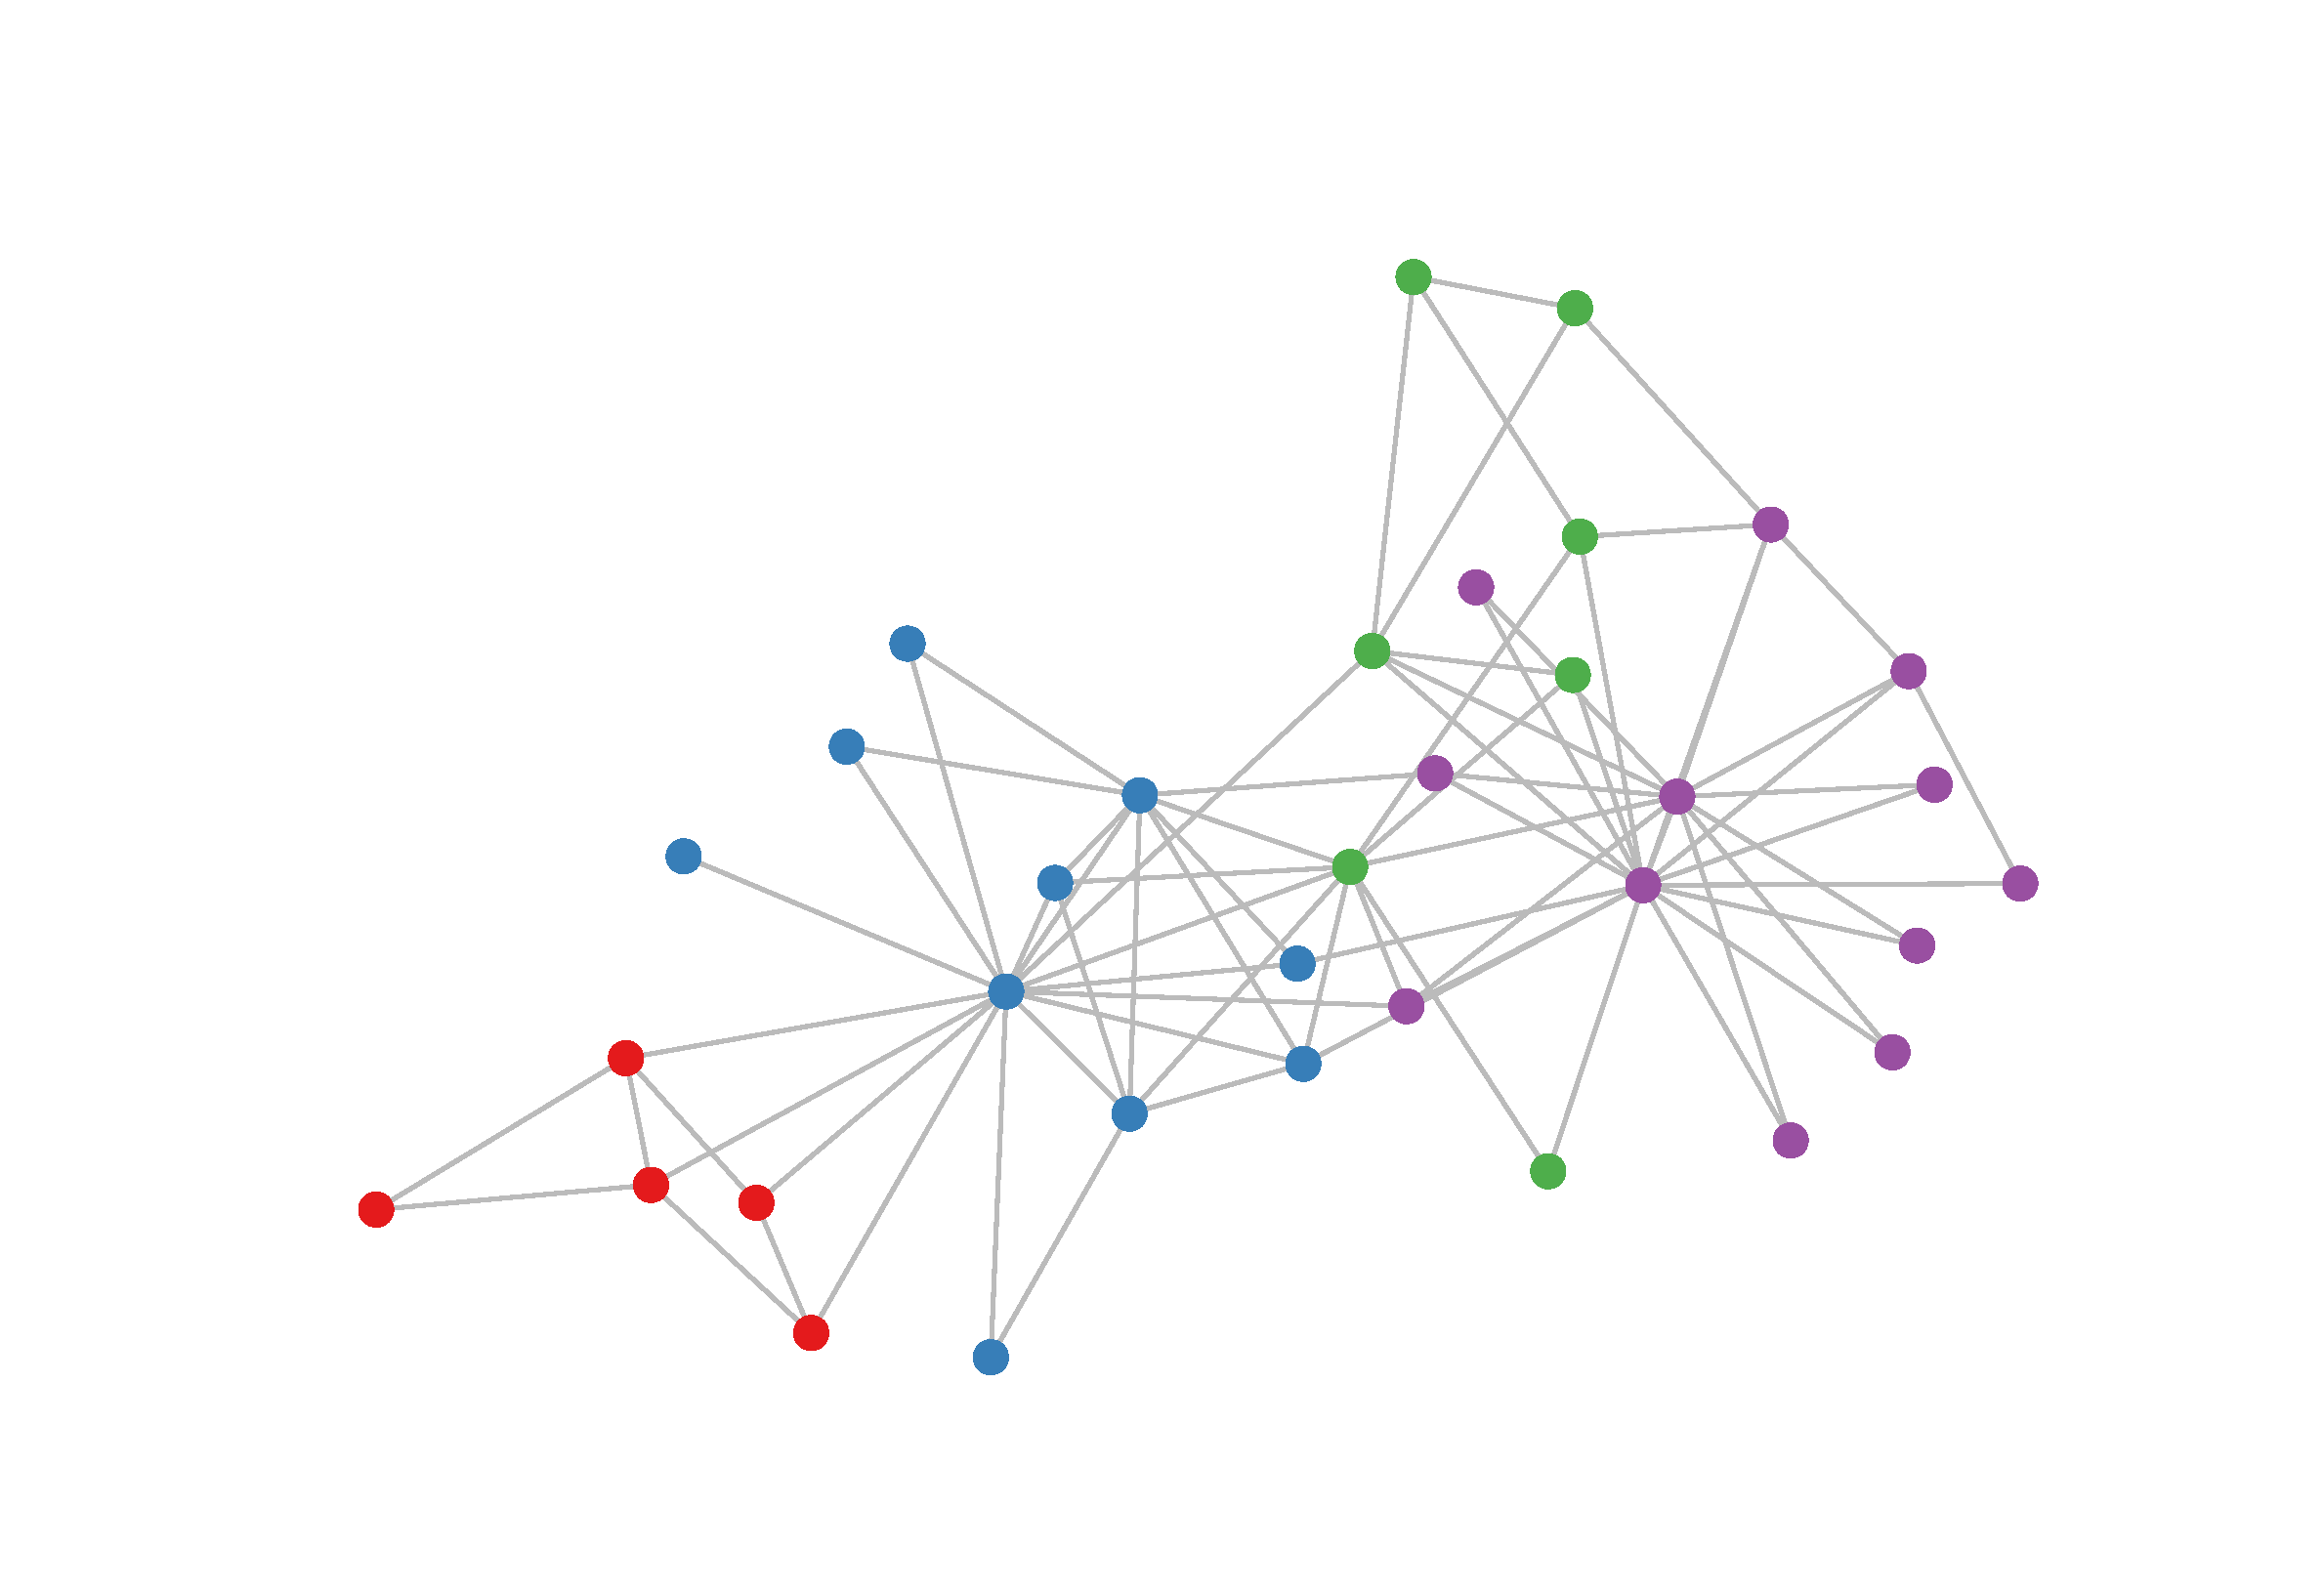
\includegraphics[width=0.95\textwidth, trim={5cm 3.2cm 4.9cm 4.4cm}, clip]{karate.pdf}
    \caption{Karate club network}
    \label{fig:karate-club-a}
\end{subfigure}%
~
\begin{subfigure}[b]{0.5\textwidth}
    \centering
    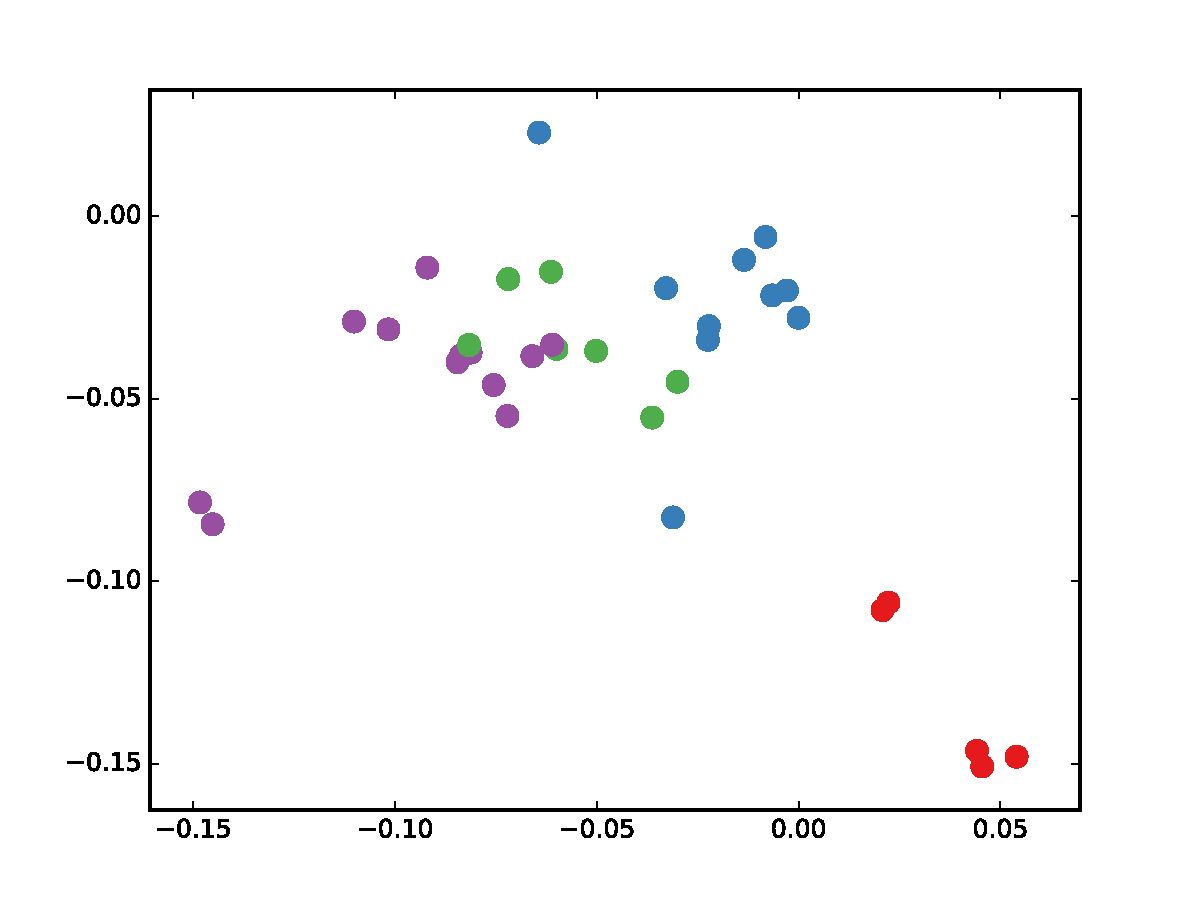
\includegraphics[width=\textwidth, trim={0 1cm 0 0}, clip]{karate_emb.pdf}
    \caption{Random weight embedding}
    \label{fig:karate-club-b}
\end{subfigure}
\caption{\textit{Left}: Zachary's karate club network \citep{zachary1977information}, colors denote communities obtained via modularity-based clustering \citep{brandes2008modularity}. \textit{Right}: Embeddings obtained from an untrained 3-layer GCN model (\eq \ref{eq:three-layer-gcn}) with random weights applied to the karate club network. Best viewed on a computer screen.}
\label{fig:karate-club}
\end{figure}

We take a featureless approach by setting $X=I_N$, where $I_N$ is the $N$ by $N$ identity matrix. $N$ is the number of nodes in the graph. Note that nodes are randomly ordered (\ie ordering contains no information). Furthermore, we choose a hidden layer dimensionality\footnote{We originally experimented with a hidden layer dimensionality of $2$ (\ie same as output layer), but observed that a dimensionality of $4$ resulted in less frequent saturation of $\tanh(\cdot)$ units and therefore visually more pleasing results.} of $4$ and a two-dimensional output (so that the output can immediately be visualized in a 2-dim plot).

Figure \ref{fig:karate-club-b} shows a representative example of node embeddings (outputs $Z$) obtained from an untrained GCN model applied to the karate club network. These results are comparable to embeddings obtained from DeepWalk \citep{perozzi2014deepwalk}, which uses a more expensive unsupervised training procedure.


\subsection{Semi-Supervised Node Embeddings}
On this simple example of a GCN applied to the karate club network it is interesting to observe how embeddings react during training on a semi-supervised classification task. Such a visualization (see Figure \ref{fig:semi-emb}) provides insights into how the GCN model can make use of the graph structure (and of features extracted from the graph structure at later layers) to learn embeddings that are useful for a classification task.

We consider the following semi-supervised learning setup: we add a softmax layer on top of our model (\eq \ref{eq:three-layer-gcn}) and train using only a single labeled example per class (\ie a total number of 4 labeled nodes). We train for 300 training iterations using Adam \citep{kingma2014adam} with a learning rate of $0.01$ on a cross-entropy loss.

Figure \ref{fig:semi-emb} shows the evolution of node embeddings over a number of training iterations. The model succeeds in linearly separating the communities based on minimal supervision and the graph structure alone. A video of the full training process can be found on our website\footnote{\url{http://tkipf.github.io/graph-convolutional-networks/}}.

\begin{figure}[htbp]
\centering
\begin{subfigure}[b]{0.5\textwidth}
    \centering
    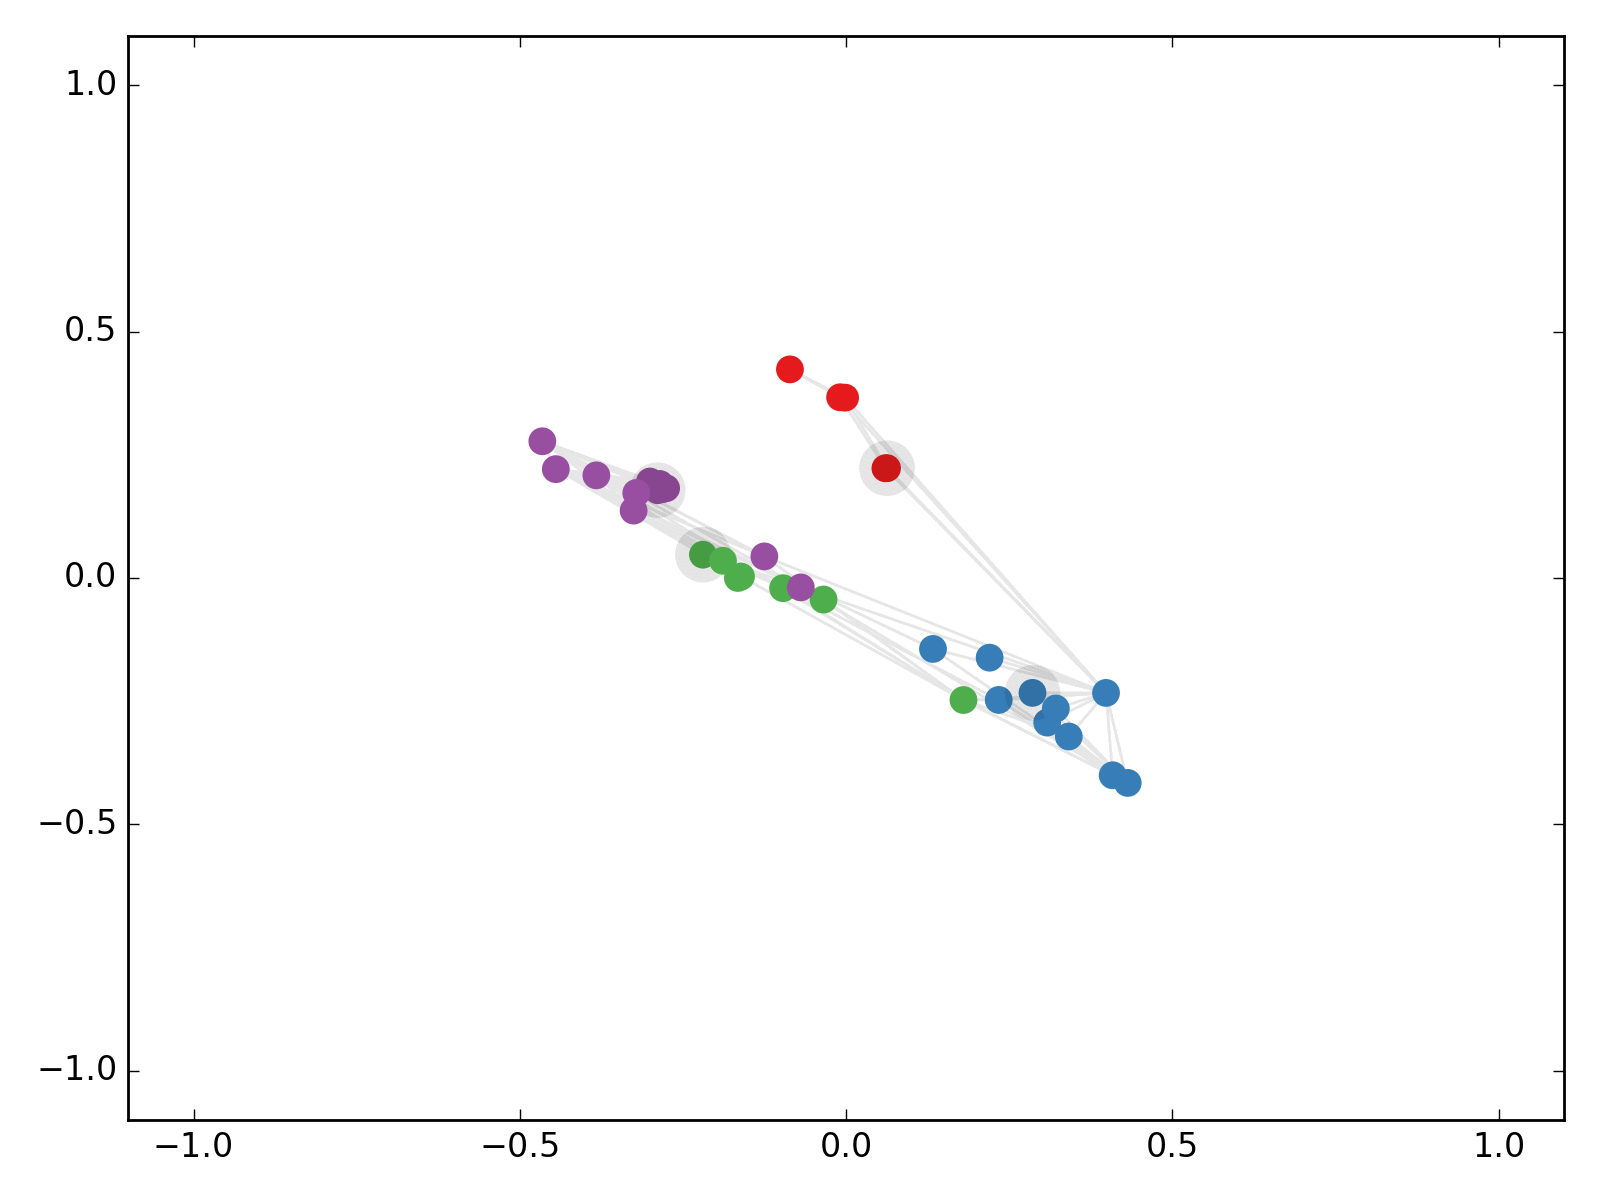
\includegraphics[width=\textwidth, trim={0 1.5cm 0 0}, clip]{anim_lines-25.png}
    \caption{Iteration 25}
    \label{fig:semi-emb-a}
\end{subfigure}%
~
\begin{subfigure}[b]{0.5\textwidth}
    \centering
    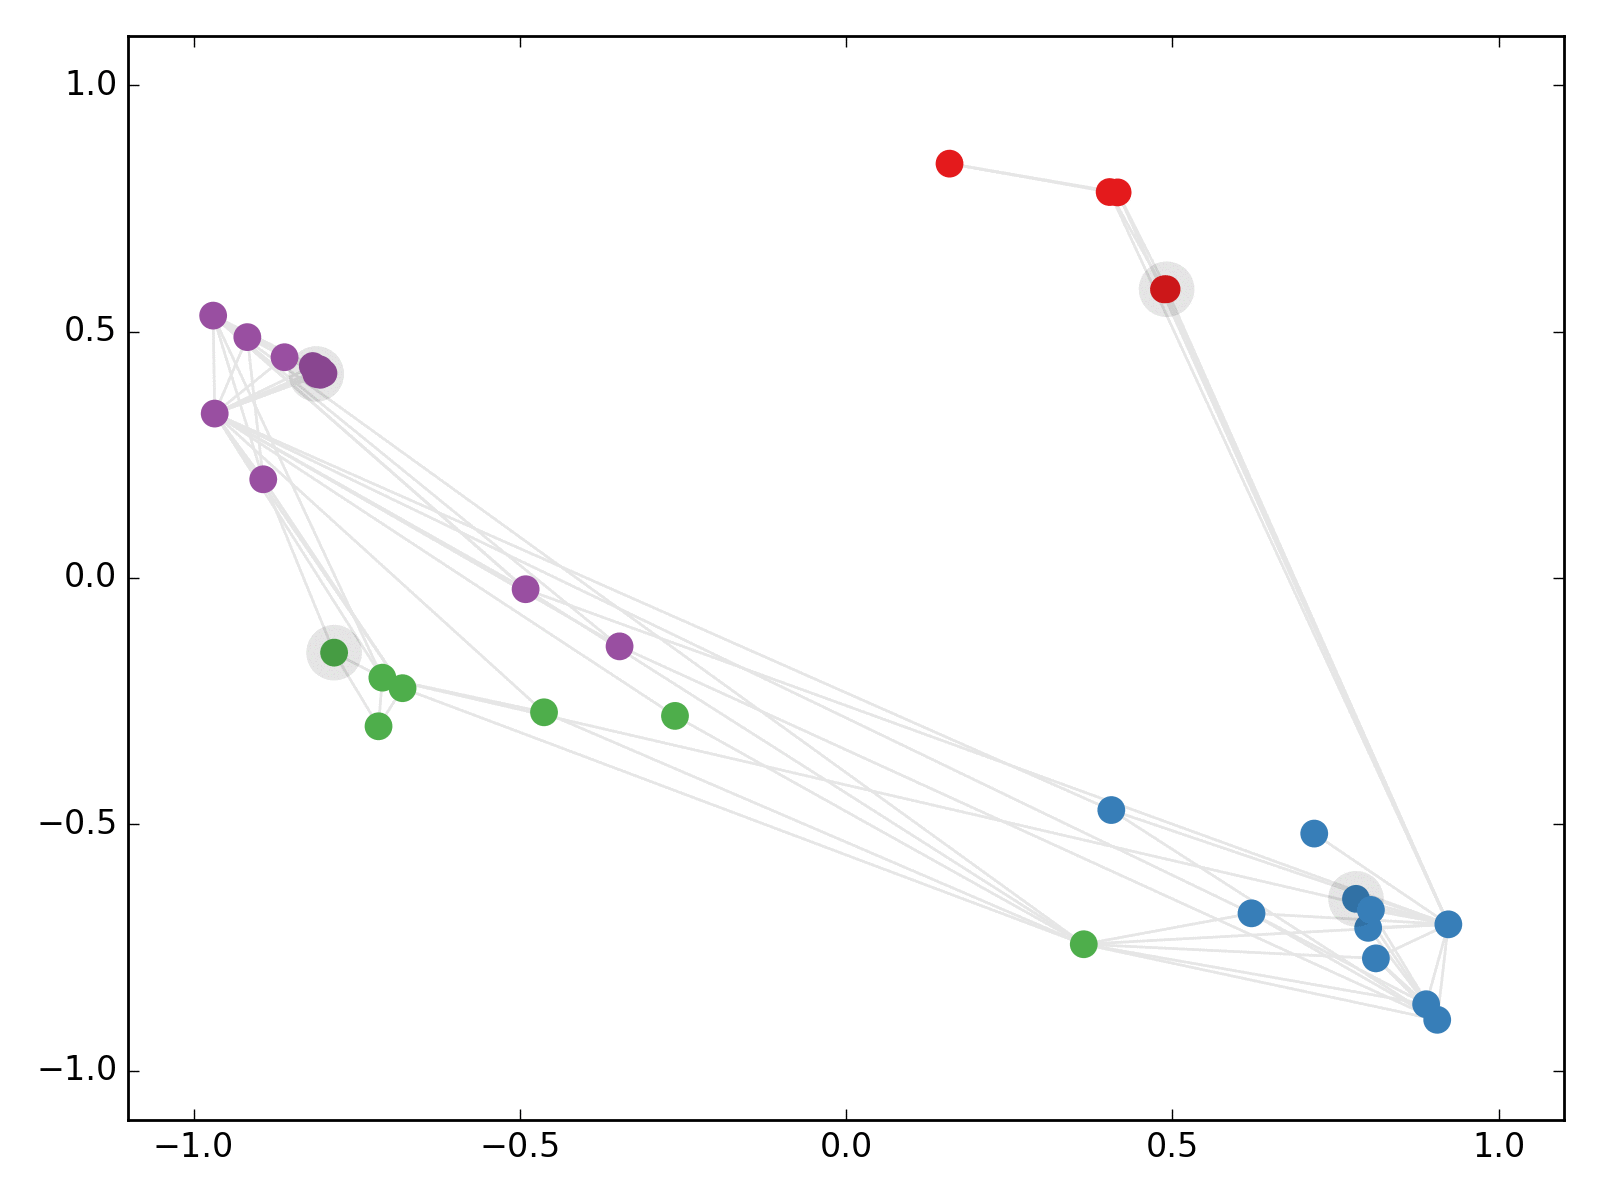
\includegraphics[width=\textwidth, trim={0 1.5cm 0 0}, clip]{anim_lines-50.png}
    \caption{Iteration 50}
    \label{fig:semi-emb-b}
\end{subfigure}%
\vspace{0.5em}
\begin{subfigure}[b]{0.5\textwidth}
    \centering
    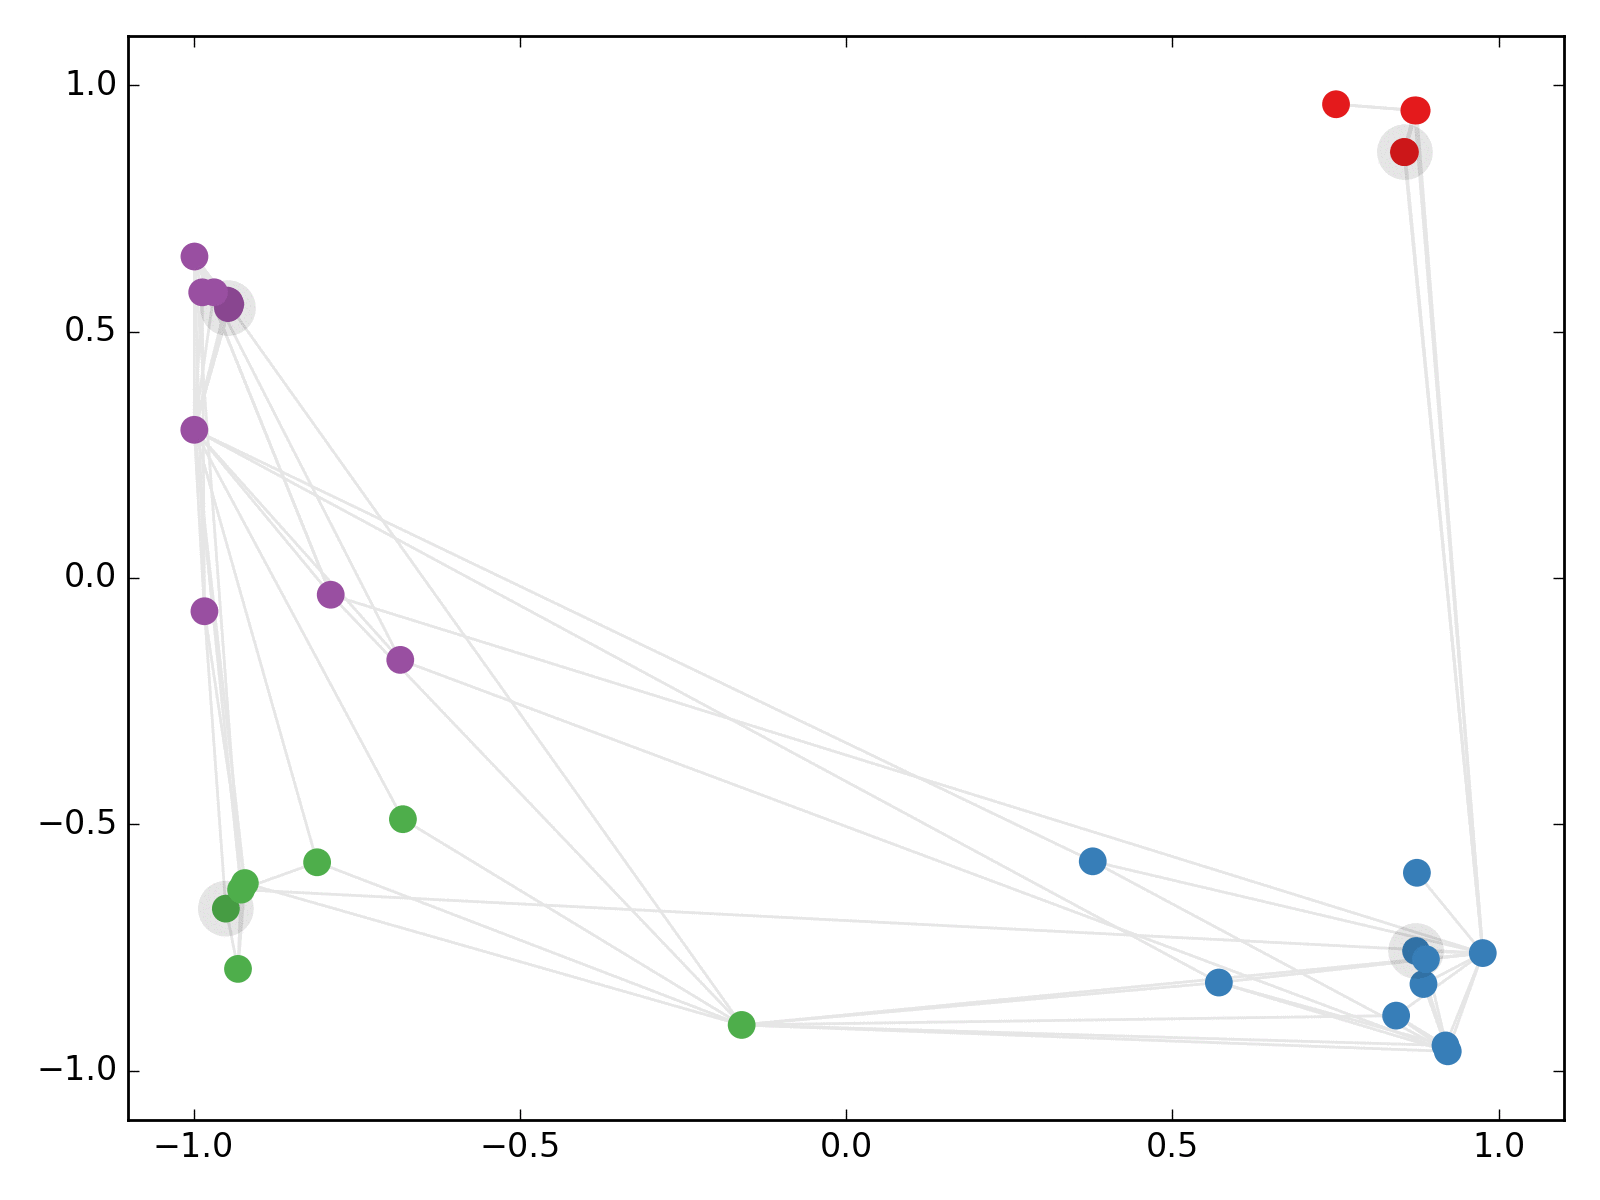
\includegraphics[width=\textwidth, trim={0 1.5cm 0 0}, clip]{anim_lines-75.png}
    \caption{Iteration 75}
    \label{fig:semi-emb-c}
\end{subfigure}%
~
\begin{subfigure}[b]{0.5\textwidth}
    \centering
    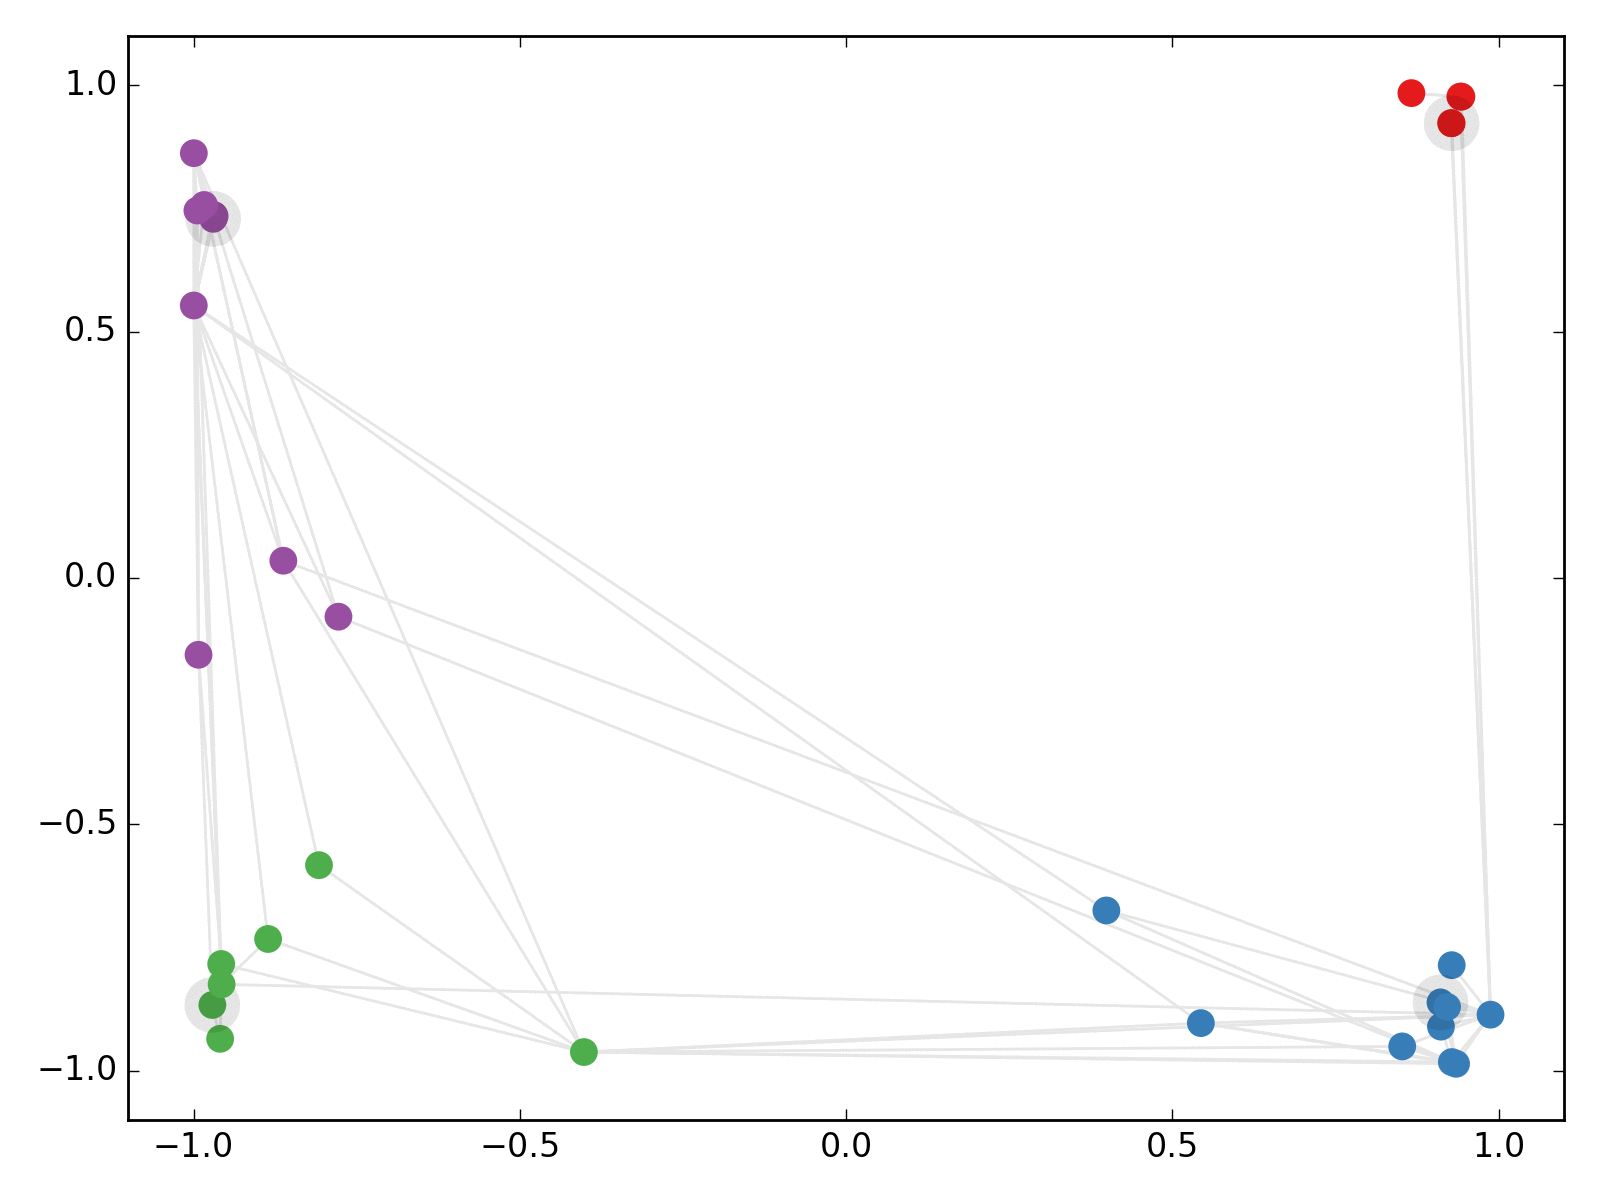
\includegraphics[width=\textwidth, trim={0 1.5cm 0 0}, clip]{anim_lines-100.png}
    \caption{Iteration 100}
    \label{fig:semi-emb-d}
\end{subfigure}%
\vspace{0.5em}
\begin{subfigure}[b]{0.5\textwidth}
    \centering
    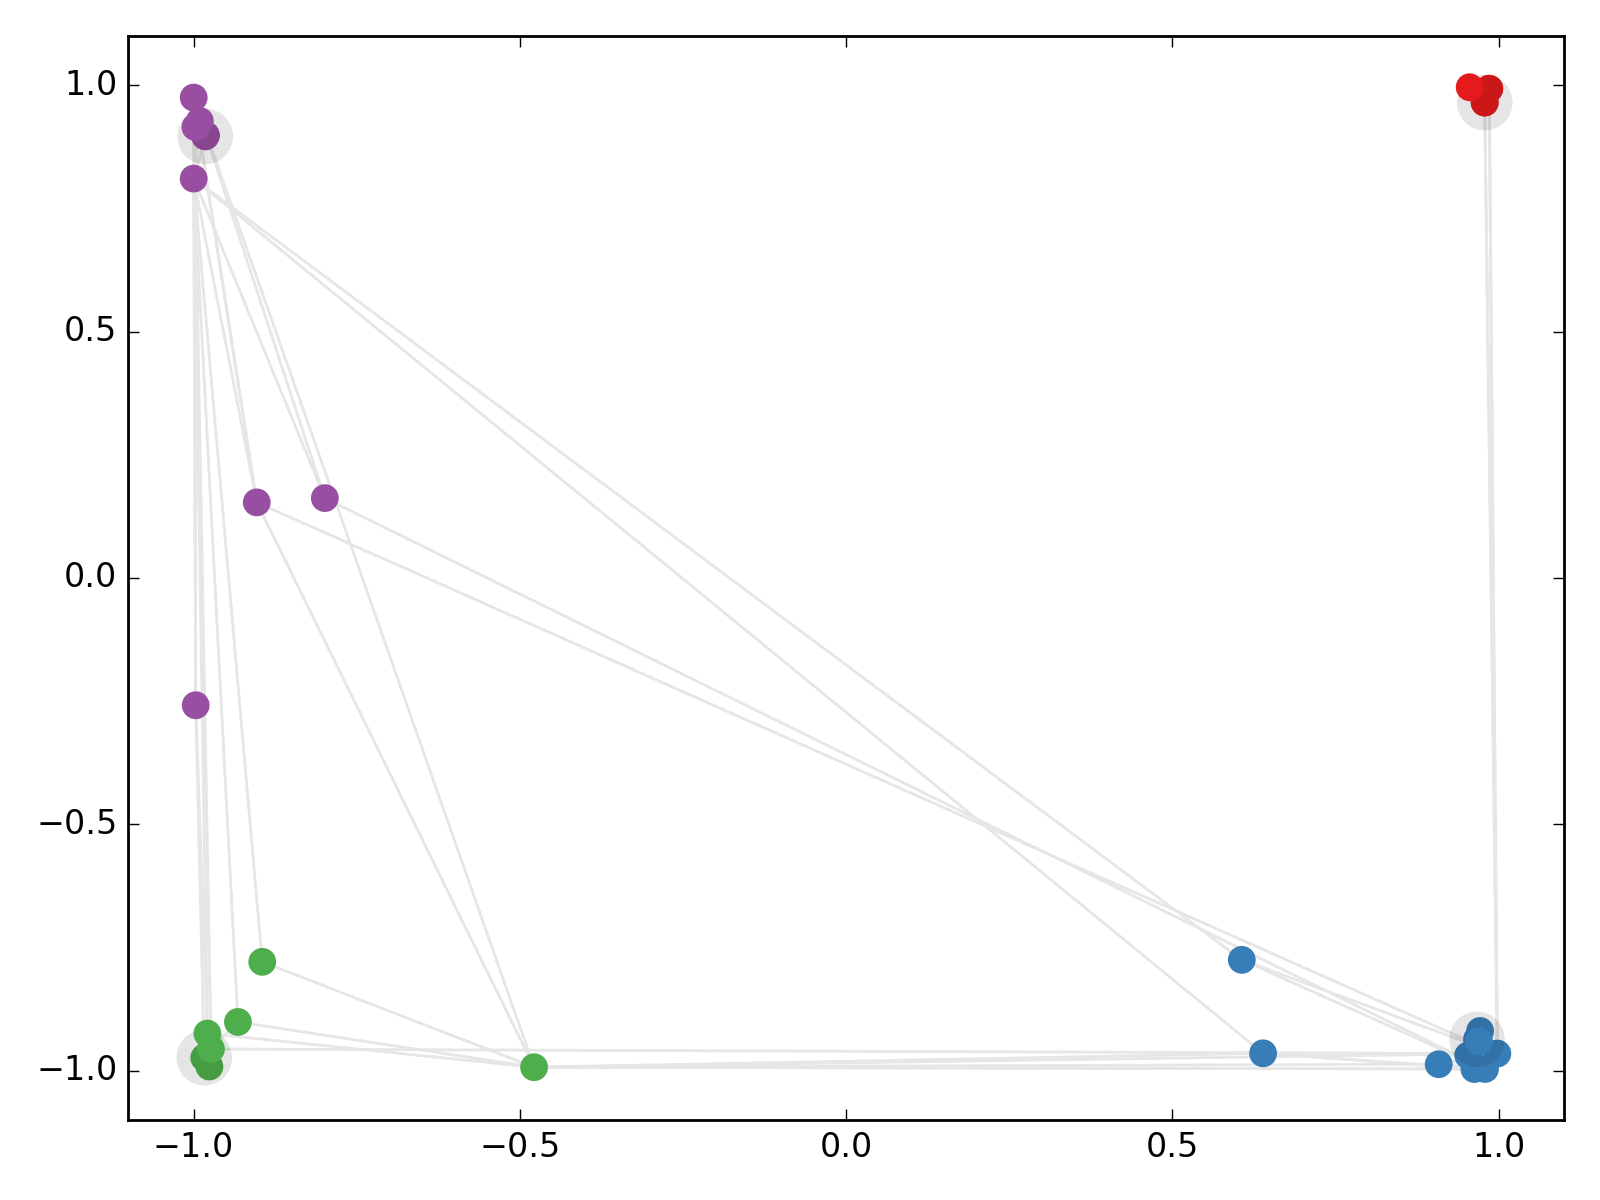
\includegraphics[width=\textwidth, trim={0 1.5cm 0 0}, clip]{anim_lines-200.png}
    \caption{Iteration 200}
    \label{fig:semi-emb-e}
\end{subfigure}%
~
\begin{subfigure}[b]{0.5\textwidth}
    \centering
    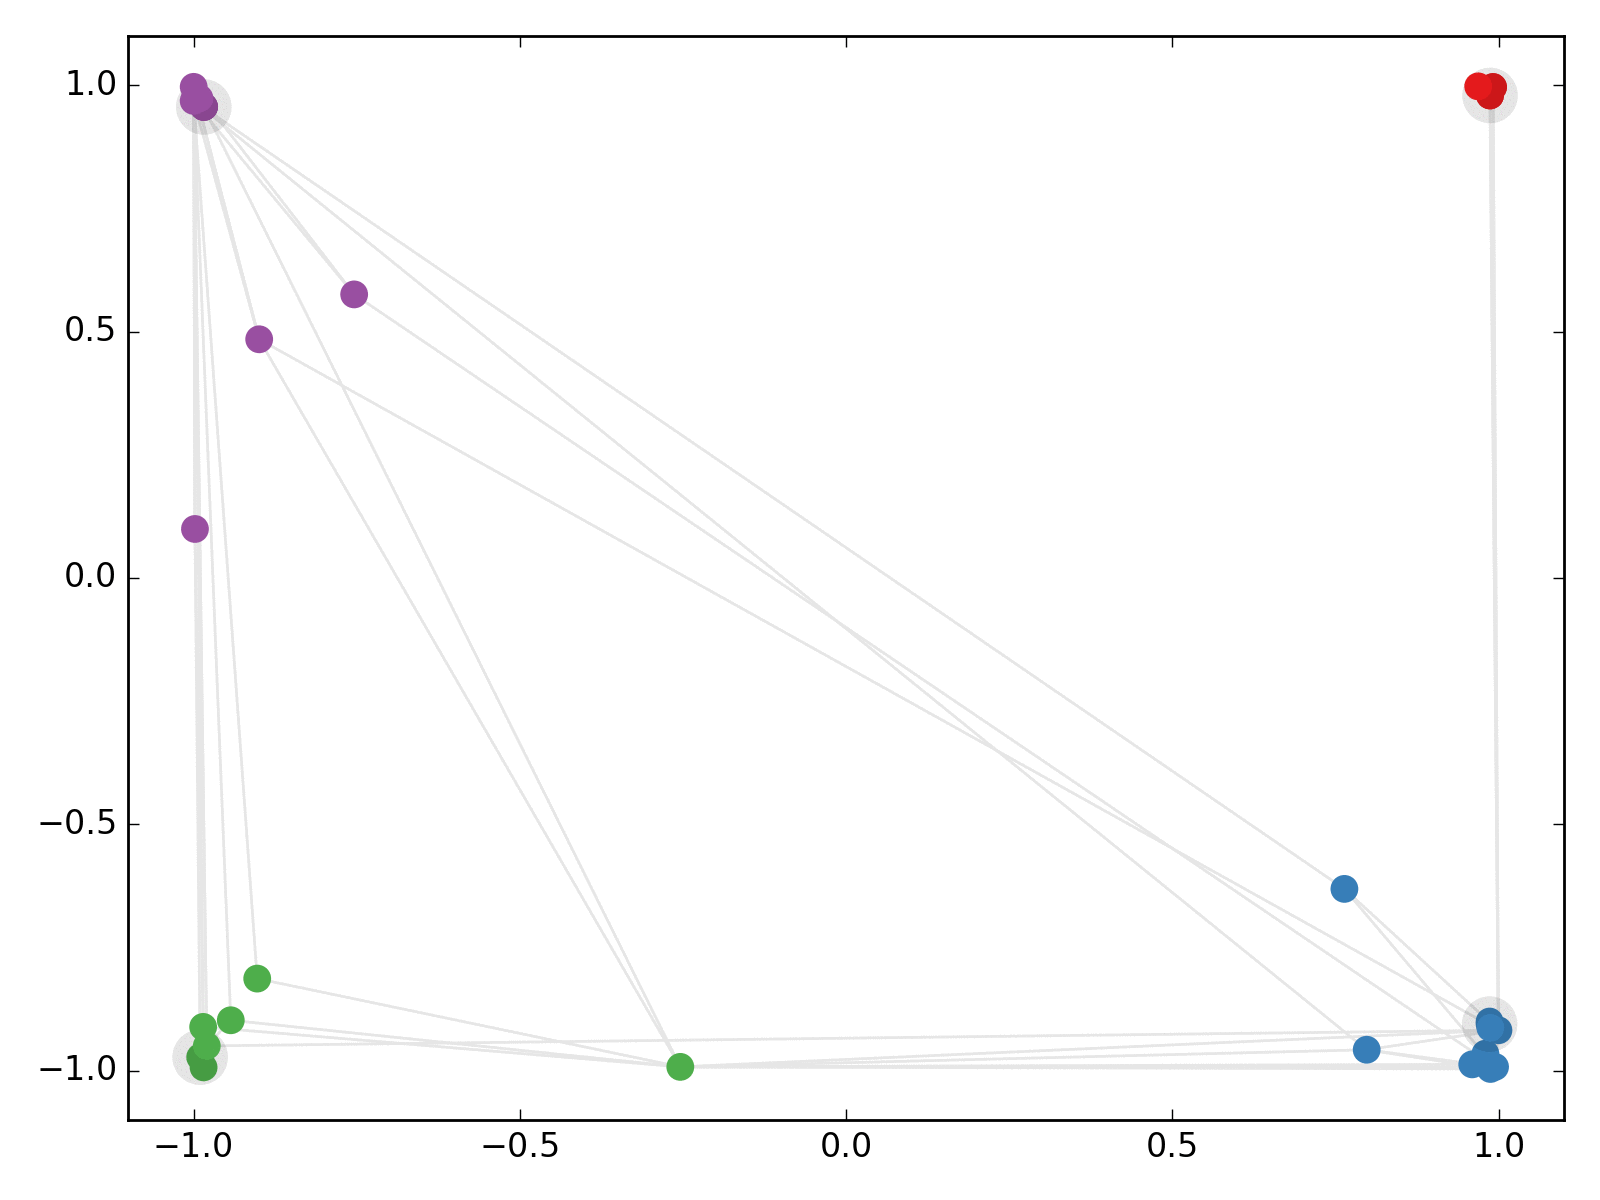
\includegraphics[width=\textwidth, trim={0 1.5cm 0 0}, clip]{anim_lines-300.png}
    \caption{Iteration 300}
    \label{fig:semi-emb-f}
\end{subfigure}
\caption{Evolution of karate club network node embeddings obtained from a GCN model after a number of semi-supervised training iterations. Colors denote class. Nodes of which labels were provided during training (one per class) are highlighted (grey outline). Grey links between nodes denote graph edges. Best viewed on a computer screen.}
\label{fig:semi-emb}
\end{figure}

\newpage
\section{Experiments on Model Depth}
\label{sec:depth}
In these experiments, we investigate the influence of model depth (number of layers) on classification performance. We report results on a 5-fold cross-validation experiment on the Cora, Citeseer and Pubmed datasets \citep{sen2008collective} using all labels. In addition to the standard GCN model (\eq \ref{eq:gcn-layer}), we report results on a model variant where we use residual connections \citep{he2015deep} between hidden layers to facilitate training of deeper models by enabling the model to carry over information from the previous layer's input:
\begin{equation}
  \textstyle
  H^{(l+1)}= \sigma\!\left(\tilde{D}^{-\frac{1}{2}} \tilde{A}\tilde{D}^{-\frac{1}{2}}H^{(l)} W^{(l)} \right) + H^{(l)} \, .
\label{eq:gcn-residual-layer}
\end{equation}


On each cross-validation split, we train for 400 epochs (without early stopping) using the Adam optimizer \citep{kingma2014adam} with a learning rate of $0.01$. Other hyperparameters are chosen as follows: 0.5 (dropout rate, first and last layer), $5\cdot 10^{-4}$ (L2 regularization, first layer), 16 (number of units for each hidden layer) and 0.01 (learning rate). Results are summarized in Figure \ref{fig:model-depth}.

\begin{figure}[htbp]
\centering
\begin{subfigure}[b]{0.33\textwidth}
    \centering
    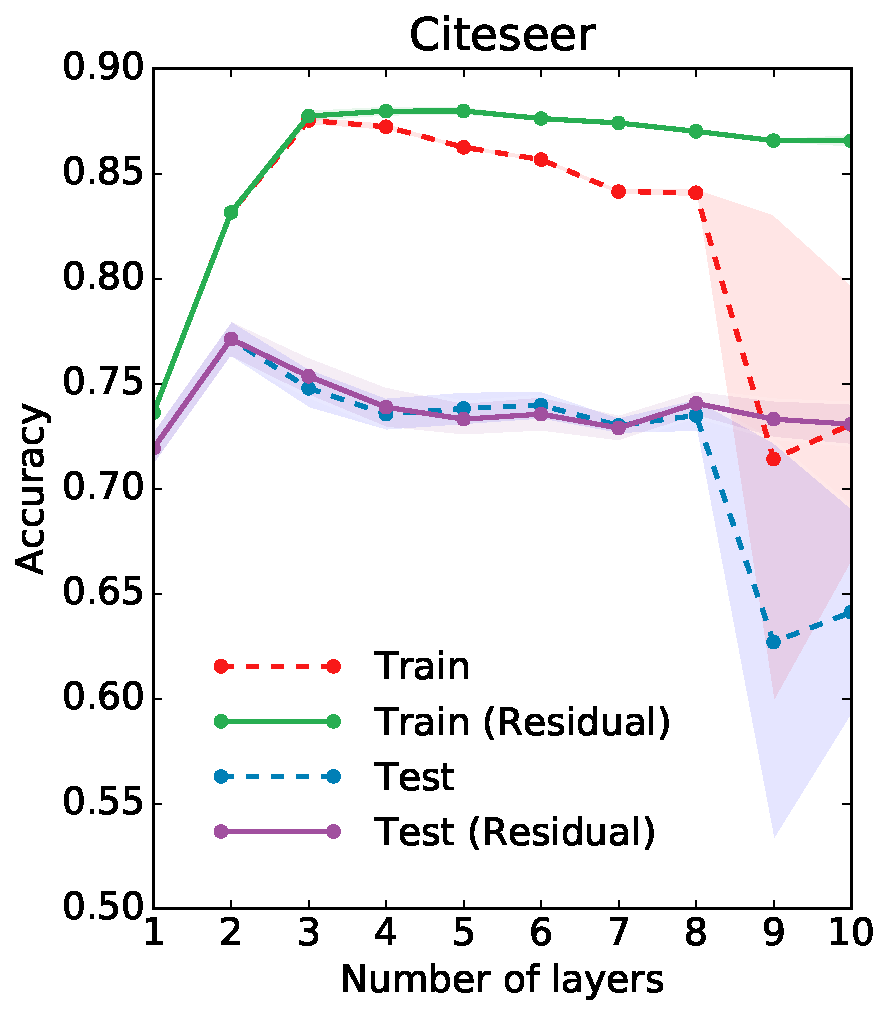
\includegraphics[width=\textwidth]{citeseer.pdf}
    \label{fig:model-depth-a}
\end{subfigure}%
~
\begin{subfigure}[b]{0.33\textwidth}
    \centering
    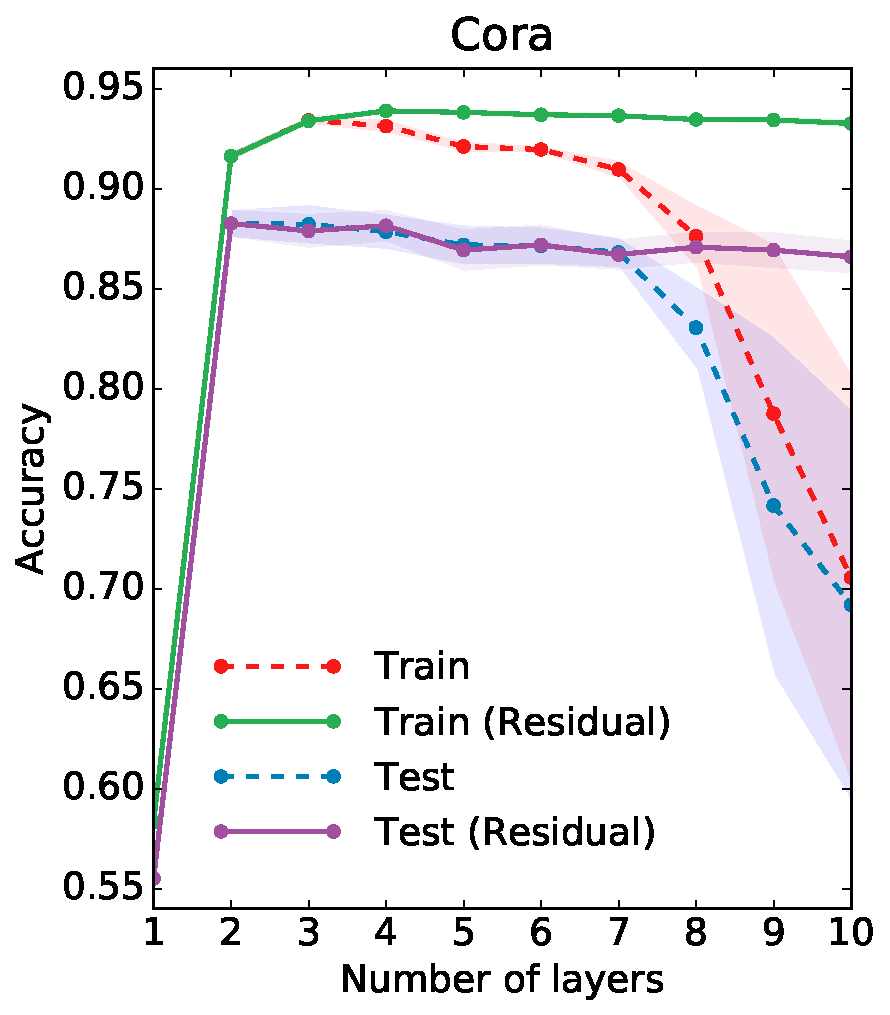
\includegraphics[width=\textwidth]{cora.pdf}
    \label{fig:model-depth-b}
\end{subfigure}%
~
\begin{subfigure}[b]{0.33\textwidth}
    \centering
    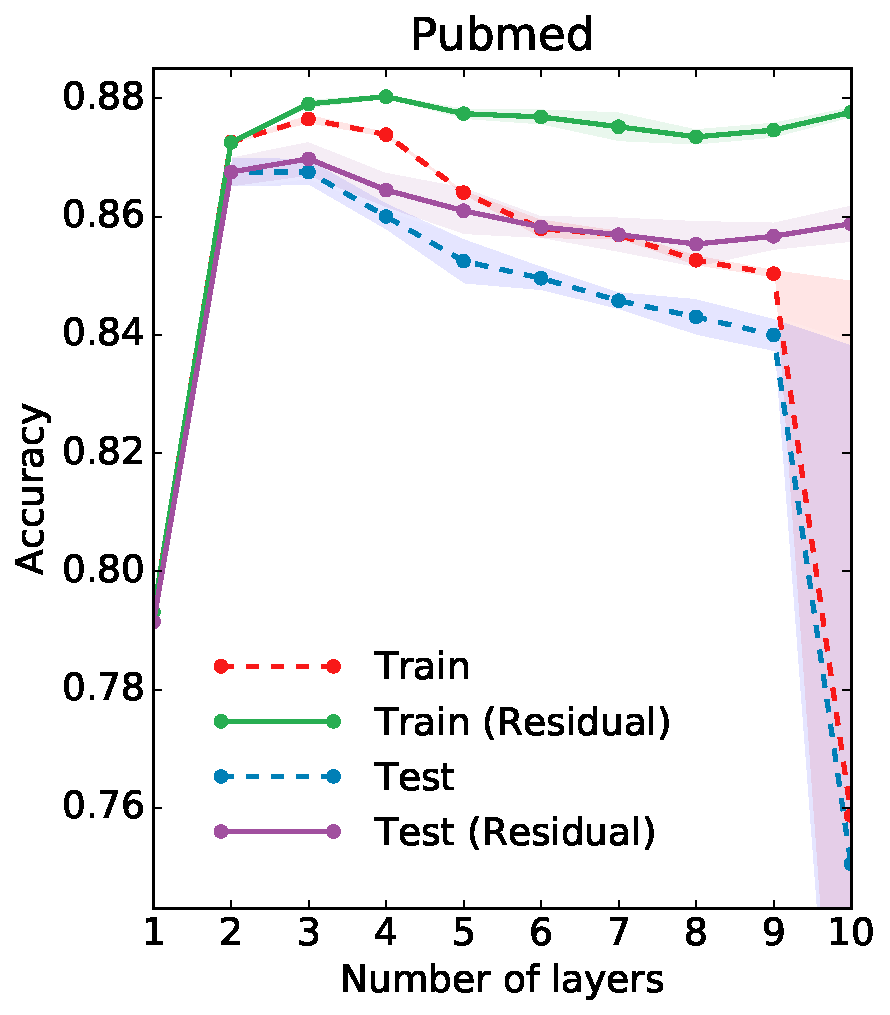
\includegraphics[width=\textwidth]{pubmed.pdf}
    \label{fig:model-depth-c}
\end{subfigure}%
\vspace{-1em}
\caption{Influence of model depth (number of layers) on classification performance. Markers denote mean classification accuracy (training \vs testing) for 5-fold cross-validation. Shaded areas denote standard error. We show results both for a standard GCN model (dashed lines) and a model with added residual connections \citep{he2015deep} between hidden layers (solid lines).}
\label{fig:model-depth}
\end{figure}

For the datasets considered here, best results are obtained with a 2- or 3-layer model. We observe that for models deeper than 7 layers, training without the use of residual connections can become difficult, as the effective context size for each node increases by the size of its $K^{\text{th}}$-order neighborhood (for a model with $K$ layers) with each additional layer. Furthermore, overfitting can become an issue as the number of parameters increases with model depth. %as the number of model parameters increases only linearly with the number of layers. Adaptive gating units as used in highway connections \citep{srivastava2015training} can alleviate this issue at the expense of introducing additional trainable parameters.

\end{document}
